\chapter{Internet measurement with RIPE Atlas}
\label{sec:ripe_atlas}
\section*{Abstract}

Starting from this chapter, the center of our study is oriented to delay and path measurements.
Same as volume data studied in Chapter~\ref{sec:pref_selec}, these measurements are readily available on client TE platforms.
However, for the sake of reproducibility, we decided to switch to measurements conducted by RIPE Atlas, a world-wide measurement platform offering open data access. We justify this choice by succinctly introducing its design philosophy and comparing it to alternative platforms.

%This decision is justified through a brief analysis on the elements of reproducibility and how RIPE Atlas satisfies them in design.
%To facilitate the discussion in later chapter concerning measurement collection, we introduce succinctly the building blocks of RIPE Atlas, its measurement methods and how a particular measurement can be identified and retrieved.

Besides reproducibility, measurement data quality is as well crucial to research credibility.
We hence study the missing measurements witnessed in measurements scheduled repeatedly. Contrary to common belief, a big part of measurements were lost while probes remained connected the to measurement infrastructure.

Further, we explore a data quality concerns specific to our TE application via unsupervised learning.
Results showcase that a part of these RTT measurements were subject to local congestion that can not be avoided with interdomain TE. This finding confirms the need for data cleaning, a process often neglected in previous practices.

Finally, we experiment several time series clustering methods to group RTT measurements with similar shape, i.e. undergoing same RTT changes.
Such RTT measurement groups, along with path measurements, can help reveal where the RTT changes come from, thus having important implication in interdomain TE.
\clearpage

\section{Reproducibility}
\marginpar{Issue with previous dataset.}
We collected traffic volume and delay data from real client networks in Section~\ref{sec:pref_selec} and developed all the studies concerning prefix selection on that dataset.
Having access to real client data increases the credibility of the discoveries made, and enhances the relevance of proposed schemes basing on these findings.
The other side of coin is that such private dataset hinder the reproducibility, a paramount feature in metrology researches.

\marginpar{What does reproducibility imply?}
The \acf{ACM} offers definition for various terms referring to different degrees of research repoducibility~\cite{acm}, ranging from repeating the same result by the same team to reproducing the same result with independent implementation of proposed methods or measurement system.
The way the measurement data is generated, stored and accessed is one key element for all these degrees of reproducibility.

\marginpar{data generation}
Previous client data come from measurements performed by proprietary TE commercial platforms~\cite{b6}.
By nature, it is against the fundamental benefit of the company to reveal the technical details on how measurements are done. 
%Even permission of disclosure granted, we as researcher more often than not do not have enough space to include such technical details in publication.

\marginpar{data storage}
Since the collected data contain sensible information, e.g. the destination prefixes clients talked to, they are required to remain on client owned platforms otherwise permission required. Due to capacity limitation and decreasing utility of old data, these measurements will not stay forever available on client servers. If measurements are allowed to be retrieved, researchers are then responsible for the storage and security of these data. 
%Server clusters in research institution may offer temporary (available till graduation) storage infrastructure, yet researchers are responsible for the security of these data. Once data compromised, researchers may face serious legal consequences.

\marginpar{access to data}
Anonymization is required it open access to private were to be granted. The process is not trivial as an appropriate balance between privacy and interpretability is hard to hit. 
%If not enough, some features of the client data can still be deduced and subject to unwanted exposure. If too much, the interpretation based on the anonymized data could become obscure and lack of credibility. 
Moreover, for better representativeness and statistical confidence, Internet measurement researches stress on large dataset over long period. 
%This inevitably increases the size of dataset. 
Maintaining the access to these large dataset is clearly not without cost. 
%However current publication reviewing process provides limited support on submitting voluminous supporting material without breaking the author/review identity anonymity~\cite{bajpai2017challenges}.

Realizing above limitations using private data, we look for measurement platforms alleviate the burden in measurement execution, storage and public access.

\section{RIPE Atlas}
RIPE Atlas is not the only Internet measurement platform that provides open data access~\cite{Bajpai2015}.
We justify this choice by first introducing RIPE Atlas. Then we summarize and highlight its features that qualify it as the best option for our research with comparison to alternative measurement platforms.

\subsection{Overview of RIPE Atlas}
\begin{figure}[!htb]
\centering
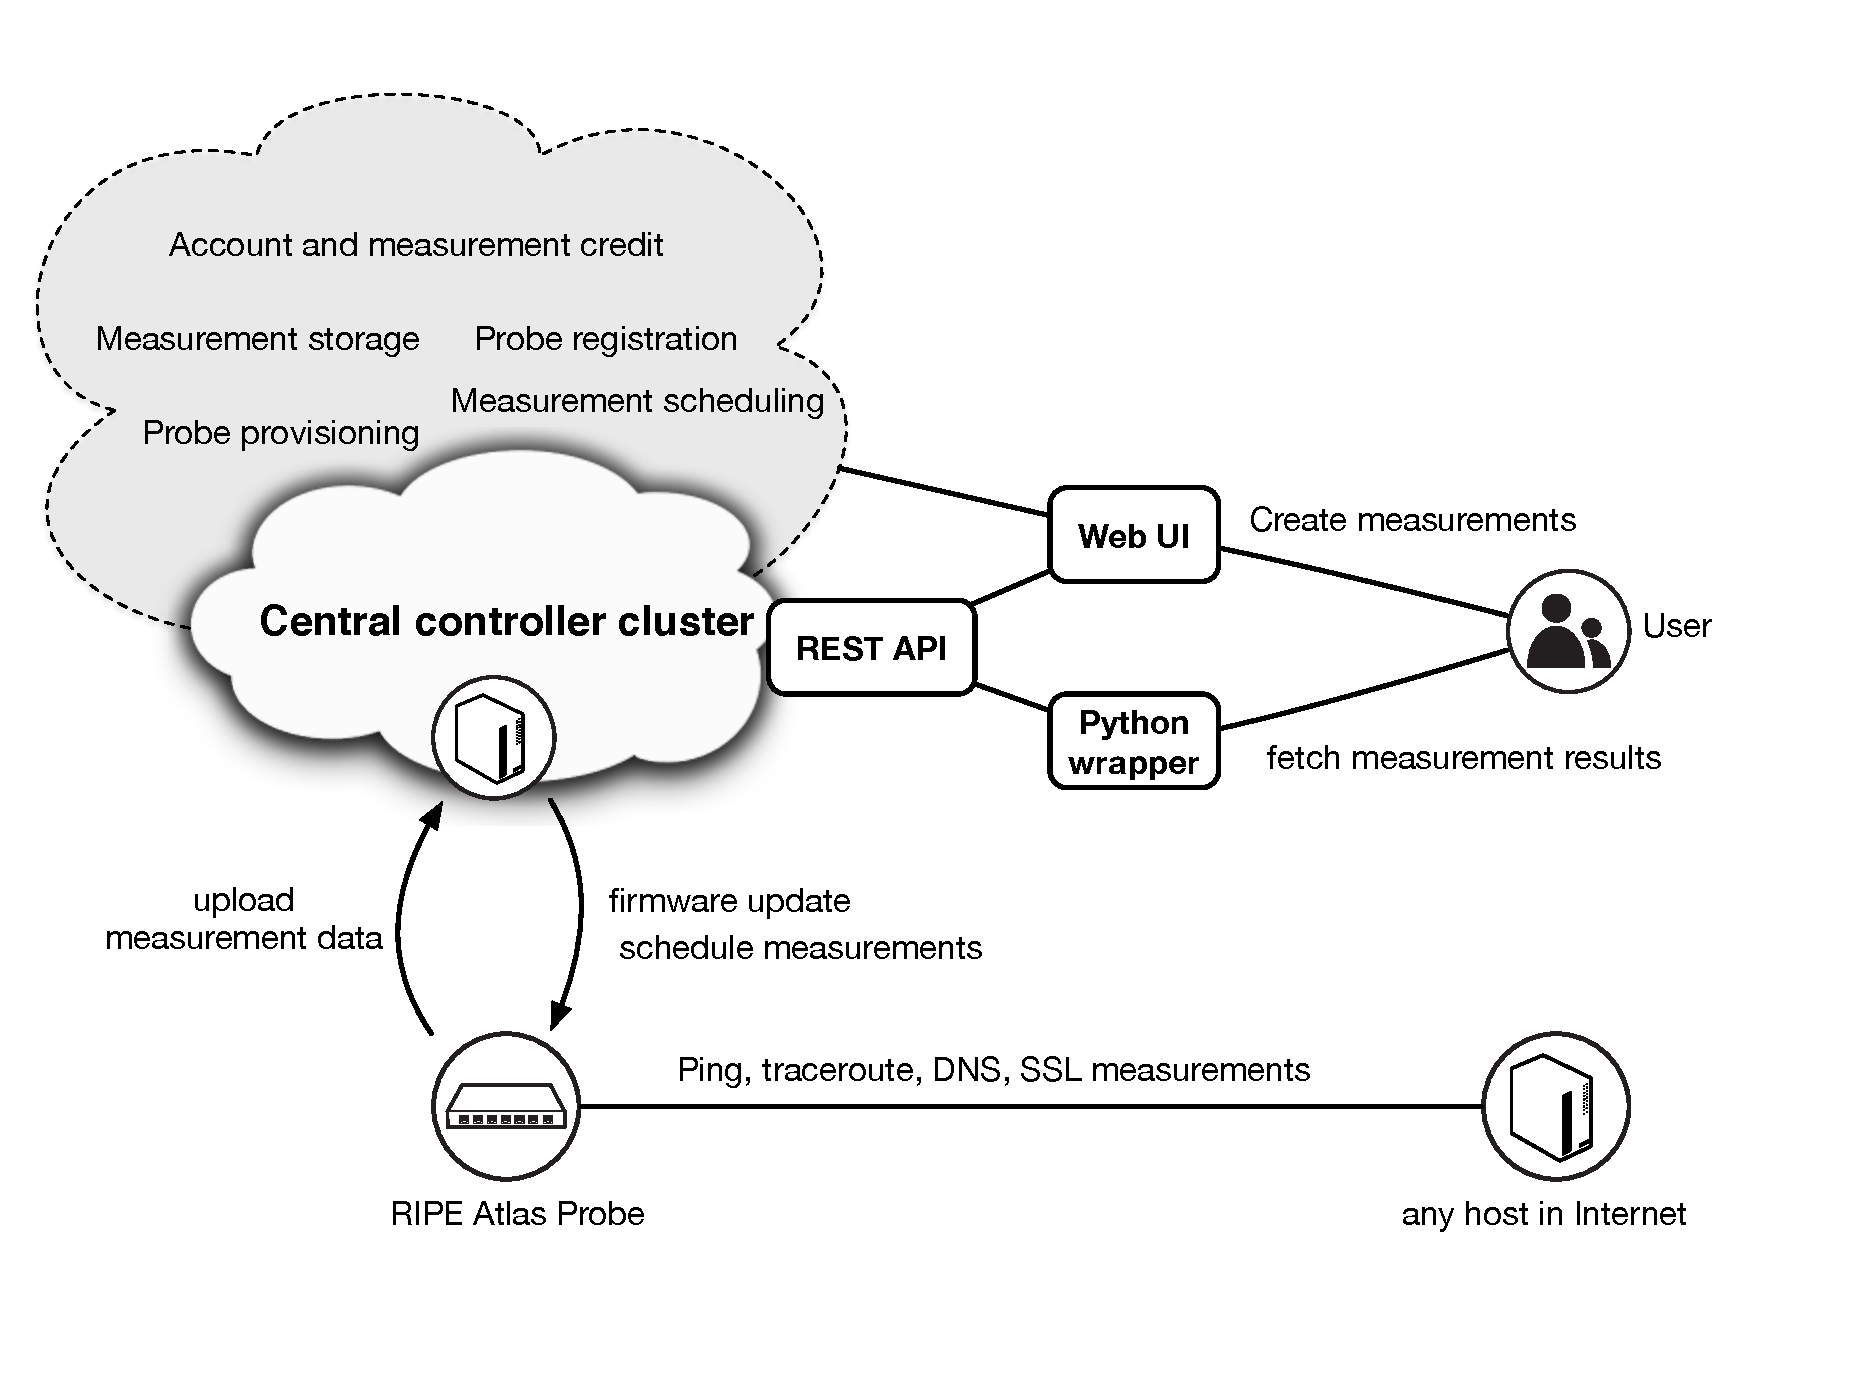
\includegraphics[width=\textwidth]{gfx/chap3/ripe_atlas_archi.pdf}
\caption{Building blocks of RIPE Atlas.}
\label{fig:ripe_atlas_archi}
\end{figure}

\acf{RIPE} Atlas is a measurement platform centrally managed by the European Internet register.
Fig.~\ref{fig:ripe_atlas_archi} sketches the architecture of the platform.
Probes are dedicated devices from which measurements are launched.
The operation system on the probes are tailored by RIPE engineers for Internet measurements~\cite{firmware}.
%These probes are distributed either by RIPE or by RIPE Atlas Ambassador~\cite{ambassador} upon demand from anyone willing to host the probe and keep it online in his network.
As of this writing (July 11, 2017), 19448 probes have been sent out and 9854 of them remain active.
All these probes, hosted in 3511 IPv4 ASes and 1286 IPv6 ASes across 181 countries, can be commanded by a single platform user to measure any destination in the Internet.

As a platform user, one does not have to connect to all these probe by him/herself to 1) create specific measurements; 2) fetch measurement results. 
One only has to interface with RIPE via programming API~\cite{atlasapi} or web page \url{https://atlas.ripe.net} to fulfill the above essential tasks along with other helpful functions such as measurement data visualization.
To that end, RIPE collects in quasi-realtime measurements from all the connected probes and stores them in its server clusters.

\subsection{Measurement types}
RIPE Atlas supports a wide range of standardized Internet measurements with configurable parameters: ping, traceroute, DNS, SSL.
%It is though not possible to run user specified measurement tools, e.g. nmnap~\cite{nmap}, scamper~\cite{luckie2010scamper} or bandwidth measurement tools, 
Ping and traceroute measurement offer the Internet delay and path information required in measurement-based TE.

Another way of classifying the measurements is via the entity of measurement creator. As shown Fig.~\ref{fig:ripe_atlas_archi}, user of the platform enjoys a great degree of 
liberty of specifying the destination, sources and time range of supported measurements. These are \acf{UDM}. Once a user defines a measurement, the central controller clusters schedules it to corresponding probes and collects the measurement results.

There exists another category of measurements called \textit{built-in measurements}~\cite{atlas}. These measurements are automatically executed by the probes without the need for controller scheduling. These measurements, originated from all probes, are mainly ping, traceroute and DNS measurements to DNS root servers and RIPE infrastructures.
In later studies, we heavily rely on these built-in measurements given their world-wide footprint, super long history records (dating back to the first connection of each probe) and low additional measurement costs.

\subsection{Describe, identify and fetch measurements}
Besides measurement type specific parameters, such as the protocol type for traceroute, following three elements are as well fundamental in describing a RIPE Atlas measurement: 1) participant probes; 2) the single measurement destination per measurement; 3) the time span of the measurement. 

Both \ac{UDM} and built-in measurements can be identified by a unique measurement ID, with which one learns the measurement meta-data, accesses data visualization provided by RIPE and eventually fetches the raw measurement results.

For example, with \url{https://atlas.ripe.net/measurements/3742863/#!openipmap}, one can have access to the path visualization of measurement $\#3742863$, where 100 probes word-wide are selected to perform one-time traceroute toward \url{www.sigcomm.org}. With \url{https://atlas.ripe.net/api/v2/measurements/3742863/results/?start=1462147200&stop=1462233599&format=json}, anyone can easily download the entire raw measurement records of this measurement.

\subsection{Advantages}
RIPE Atlas is a measurement platform designed to facilitate reproducible researches. RIPE takes care of all the engineering challenges of 1) measurements scheduling to geographically distributed probes; 2) reliable and continuous data storage; 3) public access to data; 4) simple syntax for describing, identifying measurements; 5) well documented open-source programming tools for data manipulation.

The advantages of RIPE Atlas go beyond reproducibility. Compared to perfSONAR~\cite{perfSONAR}, PlanetLab~\cite{PlanetLab} and DIMES~\cite{DIMES}, probes of RIPE Atlas, with dedicated hardware and firmware for measurement tasks, are supposed to deliver measurements that are less impacted by probe local resource sharing issues and thus better reflect the network characteristics alone.

Moreover, RIPE Atlas is rapidly gaining popularity among many non-academic networks, such as \ac{ISP}, \ac{CP} and \ac{IXP}, thanks to a wide range of monitoring applications henceforth enabled, to name a few, performance monitoring~\cite{latencymon, Rimondini2014}, anomalies detection~\cite{Fontugne2016, Padmanabhan, halo}, peering and IXP measurements~\cite{ixp, routeixp} etc. Increasing number of commercial networks host RIPE Atlas probes, providing a much richer and realistic network profile from which measurements can be initiated, compared to other alternative options.

\section{Missing measurements on RIPE Atlas}
\label{sec:miss_atlas}
Data quality is another key issue to metrology researches besides reproducibility.
Through previous studies~\cite{Holterbach2015a, Bajpai2015}, it is now known that load have obvious impacts on measurement precision and scheduling.
We focus on data completeness, another aspect of measurement quality that received less attention so far. Missing measurements can cause various undesired consequences. Apart from widening confidence interval of inference~\cite{Fontugne2016}, it requires in general methodological adaptations, e.g. in spectrum analysis~\cite{Babu2010, Luckie2014, shao2016}, otherwise biased estimation would be expected~\cite{Baraldi2010}.
%Therefore it is of relevance to question the nature of missing measurements.

One obvious reason of missing measurements is that the probe is not running (properly), e.g. power off~\cite{schedule}.
As long as a probe is powered, it tries to maintain a connection to a controller to report measurements and receive assignments as shown in Fig.~\ref{fig:ripe_atlas_archi}. 
Therefore the probe connection activity provides a good indication of the probe availability, and is used in current investigation conducted by RIPE on probe OS stability~\cite{1look, 2look, 3look}.

In order to infer other possible causes, we compared the measurement timestamps with the moments probe connects to and disconnects from a Atlas controller.
If measurement missing coincides with the probe disconnection, chances are that the probe is dysfunctional during the missing. However, if measurements are lost while the probe is well connected, something `abnormal' should be expected, beyond the known probe OS issue.

\subsection{Data collection}
We observed the RIPE Atlas platform for one month, from 2016-06-01 to 2016-07-01 UTC.
All the v3 probes first connected before the beginning date (11613 of them) are considered.
Connection events (measurement ID 7000) and built-in Ping measurements to DNS b-root (measurement ID 1010), a highly available destination, are collected~\cite{built-in}. 
Controllers and the ping destination are not within the same network.
Controller logs the moments at which probes connects to and disconnects from it.
The built-in ping measurement is scheduled on every probe at 4min interval. 
10800 ping results are thus expected from each probe within the month.
7353 probes, out of the available 11613, had Ping measurements during this period.

\subsection{Missing measurements at first glance}
\begin{figure}
\centering
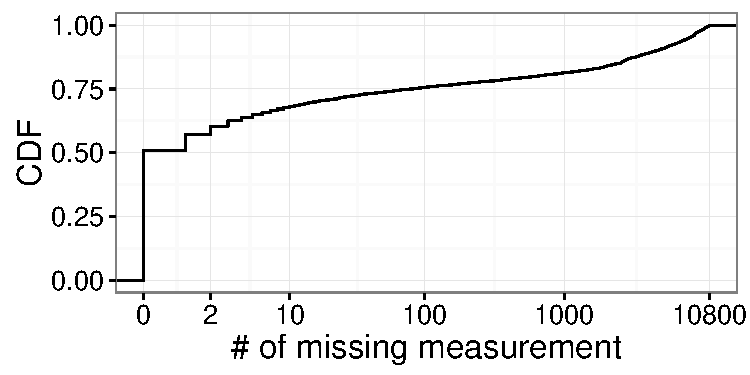
\includegraphics[width=0.7\textwidth]{gfx/chap3/missing_length_cdf.pdf}
\caption{CDF of total missing length per probe.}
\label{fig:miss_len}
\end{figure}
We deem that there are missing measurements when the time interval between two neighboring measurements are much longer than the planned value. 
Such long gaps turn out to be very close to integer times of planned interval, as a cron-like mechanism is used to run measurements at regular interval and it retakes the previous phase after interruption~\cite{source, schedule}.
This character allows quantifying the length of missing segment by the number of measurements skipped.
4440 probes  (60.4\%) miss no more than 2 datapoints, which is totally legitimate, as random jitter is added to each single measurement to avoid synchronization among probes.
For the rest, the missing length spans a wide range according to Fig.~\ref{fig:miss_len}.
1358 (18.5\%) probes miss more than 10\% of the total measurements (i.e. 72 hours over a month).

\subsection{Cross missing measurements with connection events}

\begin{figure}[!htb]
\centering
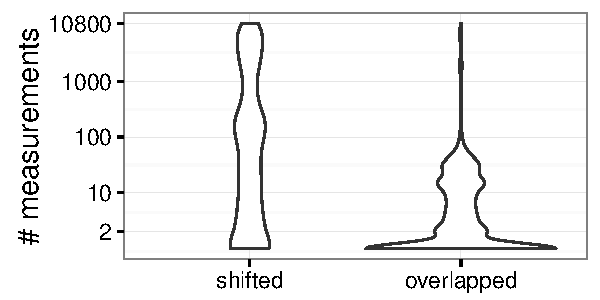
\includegraphics[width=0.6\textwidth]{gfx/chap3/len_by_ratio.pdf}
\caption{Missing length distribution.}
\label{fig:len_ratio}
\end{figure}

Several reasons may contribute to the disconnection of a probe to its controller: 1) probe not working (properly); 2) network issues preventing the connection; 3) controller not available, e.g. during maintenance~\cite{controller}. Meanwhile, the last two reasons shall not prevent a probe from performing built-in measurements, as the results can be unreachable or timeout, and be stored locally on the probe~\cite{usb}. 
That is to say, \textit{missing measurements do not necessarily occur when a probe is disconnected, but are unexpected while the probe is connected.}

\subsubsection{Overlap with connected period}
We count, for each missing segment, the number of missing measurements that occurred during a connected period.
We obtain the \textit{overlap ratio} by dividing this count by the length of missing segments. 
The distribution of overlap ratio is concentrated at the two ends, 0 and 1. 
For the convenience of illustration, we cut missing segments into two groups, one with overlap ratio $\leq0.5$, denoted as \textit{shifted}, the other with the rest, denoted as \textit{overlapped}.
Measurement missing that overlaps connected period is `unexpected'.

The two groups demonstrate different length distribution profiles, Fig.~\ref{fig:len_ratio}.
15391 missing segments are observed. 
10292 (66.87\%) missing segments are overlapped with connected period. 
They are mostly short in length. 5560 of them last no more than 2 measurements. 
One possible explanation is that these measurements are skipped due to scheduling or load issues~\cite{schedule, Holterbach2015a}.
Meanwhile, 2490 of them are equal to or longer than 1 hour, involving only 620 probes, for which we believe that the previous explanation hardly applies.
%% 620 probes ever have long overlapped missing segments, relatively a small portion.

Missing segments shifted from connected period are more likely to be long. This is possibly due to the v3 probe OS stability issue still under investigation. It is known to be responsible for long term probe disconnection and requires manual operation to recover the probe~\cite{usb, 1look, 2look, 3look}.


\subsubsection{Temporal correlation between missing measurements and connection events}

\begin{figure}[!htb]
\centering
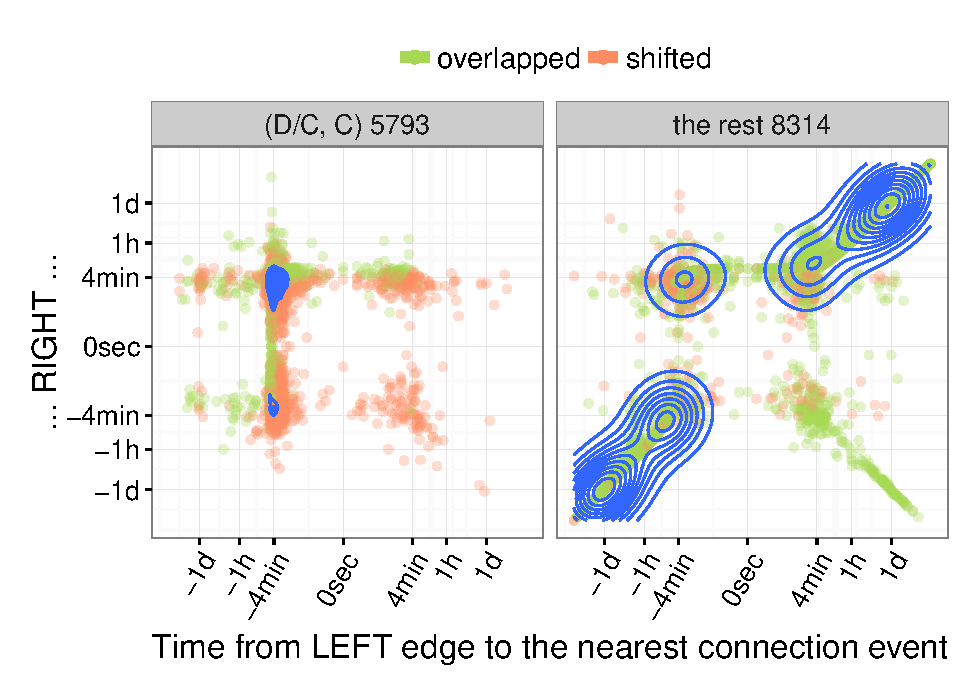
\includegraphics[width=0.98\textwidth]{gfx/chap3/all.pdf}
\caption{(D/C, C) stands for missing segments more closely correlated with disconnected period.
Number of concerned missing segments is given in the title. Negative time distance means the edge happens before the connection event and vice verse.}
\label{fig:all}
\end{figure}

To obtain a subtler view, we seek to find out: \textit{when do measurements begin to be lost and when are they recovered? Are these moments close to connection events?}

First, we define the \textit{left edge} as the last measurement before a period of measurement absence, and the \textit{right edge}, accordingly, the first measurement after recovery. 
We then calculate the time interval separating these edges and the closest connection events. We also identify the nature of these events, and mark `D/C' for disconnection, `C' for connection. 

1284 missing segments locate at the beginning or the end of the observation period. 
They are unavailable for this analysis as only one edge can be observed.
For the rest with both edges, 5793 missing segments' left edge is closer to a disconnection event and the right edge is closer to a connection event, according to Fig.~\ref{fig:all} sub-graph (D/C, C).
Judging from the density contour, last measurement most likely precedes disconnection by a Ping interval (4min), and recovery tends to take place 4 minute after the connection.
Such strong correlation with probe disconnected period indicates that probe dysfunction is probably the cause.

However, the beginning of such missing segments (D/C, C) can as well be dislocated from disconnection event.
At the left end of the graph, measurements are lost long before the disconnection, which we find `abnormal', even though the recovery is near connection.

To the right end, measurements only begin to be lost a long time after the probe is disconnected. One possible explanation is that measurements are first stored locally after disconnection from controller~\cite{usb}. Then new measurements are lost after local storage is full.

Contrary to the compact distribution in (D/C, C) sub-graph, the majority of the rest missing segments spreads along the time axis. 
The distances from left and right edge to connection events are highly correlated, suggesting that both left and right edges are on the same side of a same connection event.
We note that these measurements were mostly lost while probes were well connected, i.e. overlapped.

\subsection*{Wrap-up}
In our analysis covering a large number of probes over one month, only 60\% of v3 Atlas probes have complete measurements. Around $1/3$ missing segments appear to closely correlated to disconnected period. The probe OS stability issue might have contributed to such missings, as suggested by the heavy tail of the missing lengths.

However, the remaining $2/3$ of missing segments occurred while probes are connected. 
Half of them are no more than 2 measurements in length, and are thus likely to be caused by scheduling issues. However, around $25\%$ of this category lasts long($\geq 1h$). 

We reported the discovery to RIPE engineering team along with a specific case that they could look into.
The last reply from RIPE team confirmed that the probe we mentioned in report had ``time synchronization issues''. To help advance the investigation, we shared with RIPE team all the long missing segments identified. These exchanges can be found on the RIPE Atlas forum at \url{https://www.ripe.net/participate/mail/forum/ripe-atlas}, with tile ``Actual measurement interval much larger than planned''.

\section{Same AS path measured by different probes}
Whether the measured RTT mainly reflects the network characteristics of AS paths traversed by real traffic is a data quality concern specific in the context of measurement-based interdomain TE.

Route selection function in Fig.~\ref{fig:archi} relies on path performance measurements as input, more details in Chapter~\ref{sec:cpt_rtt}.
However, RTT measurements might be `polluted' either by non-network factors, say host-local issues such as CPU overload, or non-representative sub-AS level network issues can not be optimized with interdomain TE, say local congestion within the destination prefix.
However, none of these previous works on measurement based inter-domian TE~\cite{Goldenberg2004, Akella2008} has realized the importance of this problem.

This data quality issue gives rise to a series of questions: if we measure over a period of time a same AS path with multiple different RTT measurements toward different hosts in the destination prefix, what will these RTT time series look like? Will they have similar characters? If not, how can we pick out the ones fit best for our TE uses?
We try to answer to these questions by performing clustering over a such set of RTT time series, in the purpose of automatically revealing their inherent structures.

\subsection{Data collection}
We emulated such RTT measurements between two ASes, the local client AS (one host) and one destination AS (multiple hosts) with RIPE Atlas built-in measurements $\#1006$ and $\#5006$.
They are respectively IPv4 ping and traceroute measurements from all Atals probes to m.root-servers.net (202.12.27.33). 
Ping measurement is scheduled at 240 sec interval, while traceroute at 1800 sec.
120 RIPE Atlas probes within AS3215 are selected to construct our database.\footnote{The 120 probes are the same ones in user-defined measurement \#2427397 with open access to all.}
We assumed that all probes hit the same DNS root server clusters as the AS-level path toward the destination (m-root) is the same, since the only upstream AS for AS3215 is AS5511, the backbone of a French \ac{ISP}. Time window for the data collection ranges from 2015-09-28 10:00:00 UTC to 2015-09-29 12:00:00 UTC.

We cleaned the data collected, with following steps:
\begin{itemize}
\item Remove probes with unstable connection to the Atlas platform. (Short total length, multiple missing segments~\ref{sec:miss_atlas});
\item Remove probes suffering from obvious hardware or local network issues. (high packet loss, or error flag found in measurement results).
\end{itemize}

We then consider only 100 common probes in both ping and trace traces remained after cleaning.
All valid probes considered, the average IP hop number to the destination, m-root server, is 9. 
For the traceroute data set, we decided to concentrate on the first 3 hops (which should cover the access network). As a consequence, the traceroute data set are further cut into 3 parts, where each contains the RTT time-series till the corresponding hop.

To sum up, we fabricated four RTT time series data sets, on which we performed time series clustering:
\begin{itemize}
\item \texttt{pingData}, end-to-end RTT time series;
\item \texttt{traceData1}, RTT series till the first hop;
\item \texttt{traceData2}, RTT series till the second hop;
\item \texttt{traceData3}, RTT series till the third hop;
\end{itemize}

\subsection{Clustering RTT series in feature space}
\label{sec:cls_ft}
Generally speaking, a time series clustering approach can be decomposed into three parts: data representation, distance measure and clustering algorithm~\cite{Aghabozorgi2015}. 
Due to its high dimension, time series is seldom used in its raw form, whence data representation.
Common approaches include dimension reduction~\cite{Elhamifar2013}, pattern extraction~\cite{Ulanova2015}, etc.
Distance measure quantifies the similarity/dissimilarity of two time series. Finally, clustering algorithm defines the procedure of grouping time series based the distances calculated on their data representation space.
For each of these components, multiple possibilities exist. However, it is not clear which ones in combination could be the best fit for RTT measurements. 

In this section, we extracted a set of features listed below from each individual time-series and used in actual clustering. 
The advantage of such data representation is that it first largely reduces the data dimension. Thanks to that, data set is more suitable to classic partitioning clustering methods, like k-means and k-medoids (also known as \acf{PAM})~\cite{Lin2003}.
Second, it is able to depict the data set from multiple aspects that are not evident with the raw form. 
%However, the clustering results could be biased by the selection of features.
Before clustering, each feature is z-normalized (zero mean and unit variance).
%so that result is not biased towards features with big value and high variance.
%%% At last I understood !!! Eureka. 

Following features are used in this work:
\begin{description}
\item[Power spectral density] is calculated using PyEgg~\cite{Bao2011} and cut into three bins relative to sampling/measurement frequency, $(0, 1/12], (1/12, 1/6]$ and $(1/6, 1/2]$. Each of the bins individually functions as a feature.
\item[Sampling Entropy] proposed by Richman and Moorman~\cite{Richman2000} quantifies the regularity or predictability of a time series. In calculation~\cite{Bao2011}, we used an embed dimension of 2 and a tolerance of 15 msec.
\item[Number of changes] counts the number of times where the difference between two consecutive RTT measurements is greater than 15 msec. %We did not use change detection methods that adapt to mean and deviation level of a window in the past, e.g. those based on z-score, for we assert that an absolute RTT change more than 15msec is significant, regardless of the mean and $std$ of an RTT trace. 
\item[Range] is the difference between the maximum and the minimum values of an RTT series.
\item[Mode] is the value most frequently present in a time-series.
\item[Mean] the first-order moment, describes the overall RTT level.
\item[Standard deviation] is derived from the second-order moment, describes how close measurements are to the mean.
\item[Skewness], the third-order moment, describes the lack of symmetry of RTT values observed around the center point of histogram, mode.
\item[Kurtosis], the fourth-order moment, describes whether the histogram of observations are peaked or flat relative to a normal distribution.
\end{description}
With RTT time series represented in the above feature space, we simply use \acf{ED} to measure the distance between two RTT time series.

\iffalse
\begin{figure}[!htb]
    \centering
    \begin{subfigure}[b]{.7\textwidth}
	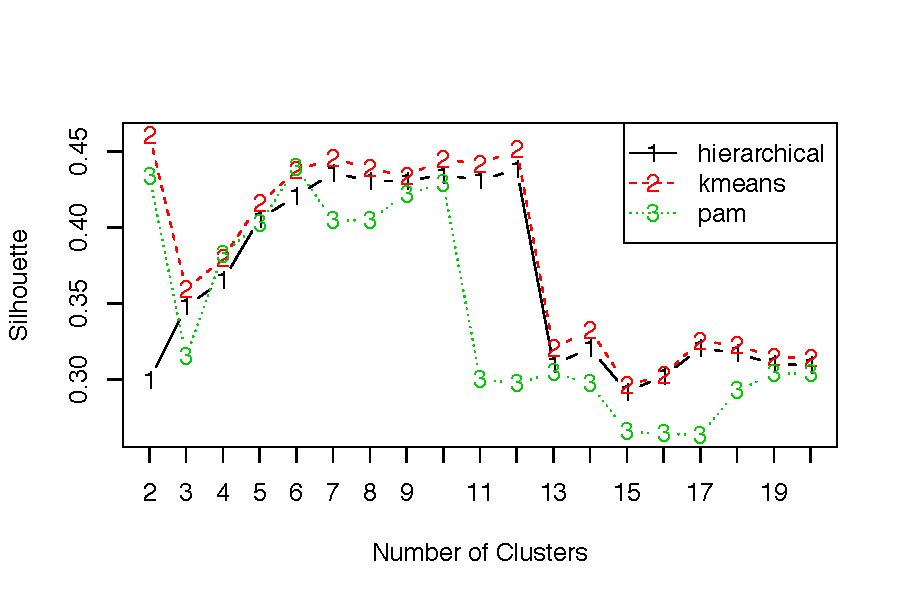
\includegraphics[width=\textwidth]{gfx/chap3/pingSil.pdf}
	\caption{\scriptsize \texttt{pingData}}
	\label{fig:pingSil}
	\end{subfigure}
	\begin{subfigure}[b]{.7\textwidth}
	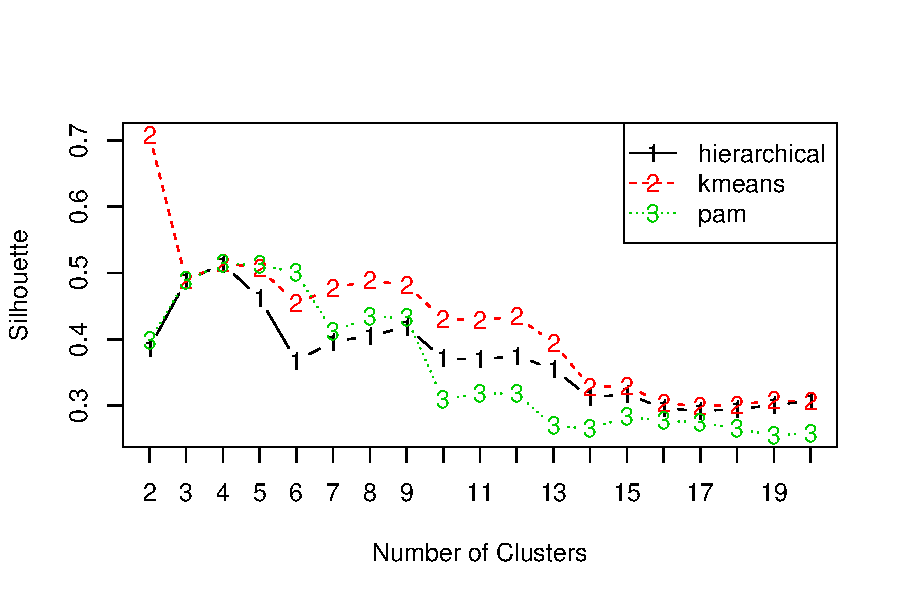
\includegraphics[width=\textwidth]{gfx/chap3/traceSil1.pdf}
	\caption{\scriptsize \texttt{traceData1}}
	\label{fig:traceSil1}
	\end{subfigure}
	\begin{subfigure}[b]{.7\textwidth}
	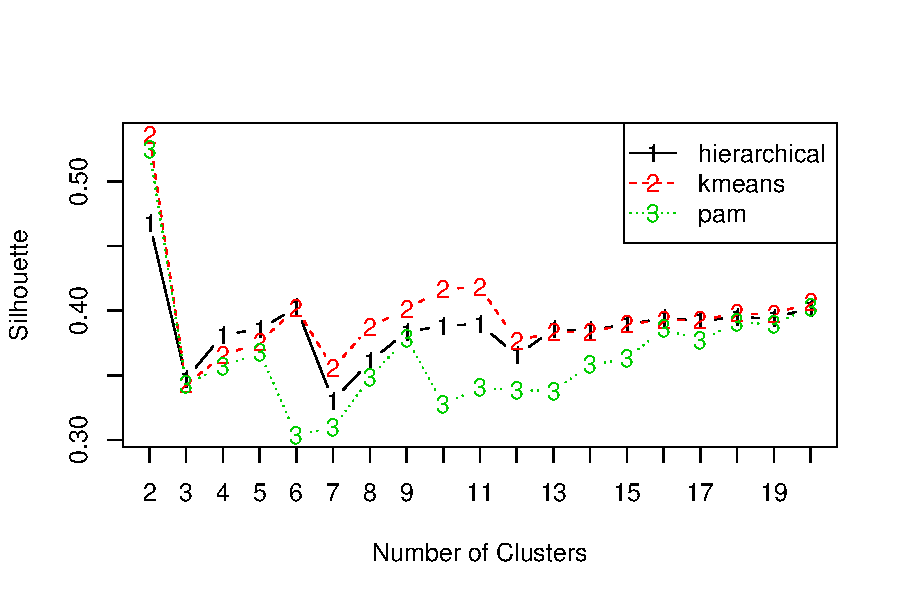
\includegraphics[width=\textwidth]{gfx/chap3/traceSil2.pdf}
	\caption{\scriptsize \texttt{traceData2}}
	\label{fig:traceSil2}
	\end{subfigure}
	\begin{subfigure}[b]{.7\textwidth}
	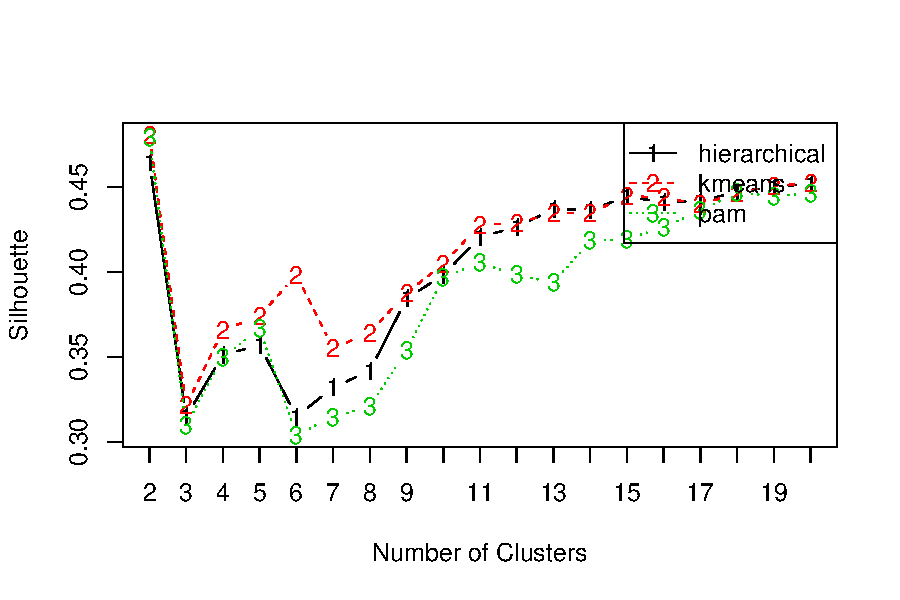
\includegraphics[width=\textwidth]{gfx/chap3/traceSil3.pdf}
	\caption{\scriptsize \texttt{traceData3}}
	\label{fig:traceSil3}
	\end{subfigure}
\caption{ASW (Average Silhouette Width) using different clustering algorithms when varying number of clusters.}
\label{fig:sil}
\end{figure}
\fi

\begin{figure}[!htb]
\centering
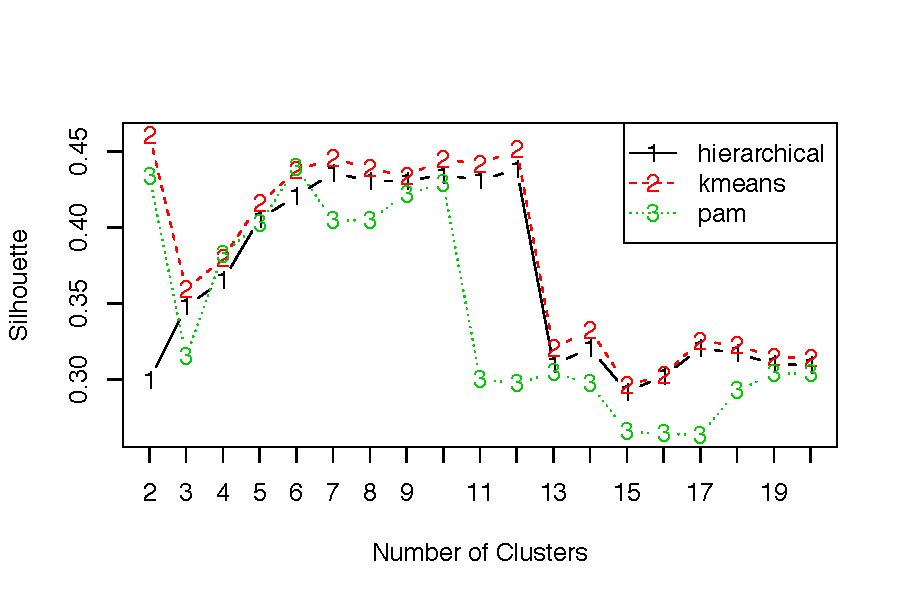
\includegraphics[width=.9\textwidth]{gfx/chap3/pingSil.pdf}
\caption{\ac{ASW} achieved on \texttt{PingData} using different clustering algorithms when varying number of clusters.}
\label{fig:pingSil}
\end{figure}

\marginpar{Which cluster method is the most appropriate?}
Several clustering algorithms are available. 
In order to choose the one that fits best to our data set and decide the most appropriate cluster number, we use \acf{ASW}~\cite{Rousseeuw1987} to evaluate the quality of resulted clusters. 
It takes value in the range of $[-1,1]$. 
\ac{ASW} of a certain achieved cluster is a measure of how tightly all the data points in the cluster are grouped together. 
While the \ac{ASW} over the entire dataset, is a measure of how appropriately the entire data set has been clustered. For a single clustering method, we can find out what is the cluster number k that this algorithm is most confident of by picking the k offering the biggest \ac{ASW}. Across two different clustering algorithms, we could tell which one performs better by comparing the \ac{ASW} of resulted clusters, i.e. a better clustering result shall have a bigger \ac{ASW} value.

Following clustering algorithms are tested: hierarchical clustering with Ward linkage, k-means and \ac{PAM}.
Dataset-wide \ac{ASW} are visualized in Fig.~\ref{fig:pingSil}. We can see that for \texttt{PingData}, k-means algorithm with $k=2$ offers relatively confident clustering results. 
This observation holds as well true for traceroute data sets.
Hence, such settings are used in the rest of this study.


\subsection{Clustering result interpretation}

\begin{table}[!htb]
\centering
\footnotesize
\setlength{\tabcolsep}{0.5em}
\begin{tabular}{l|ccc|ccc|ccc|ccc}
\toprule
\multirow{2}{*}{\# cls} & \multicolumn{3}{c|}{\texttt{pingData}} & \multicolumn{3}{c|}{\texttt{traceData1}} & \multicolumn{3}{c|}{\texttt{traceData2}} & \multicolumn{3}{c}{\texttt{traceData3}}\\
& size & dist. & AWS & size & dist. & AWS & size & dist. & AWS & size& dist. & AWS\\
\midrule
1 & 25 & 4.37 & 0.23 & 93 & 3.98 & -0.21 & 76 & 3.02 & 0.41 & 31 & 4.35 & 0.07\\
2 & 75 & 2.61 & 0.54 & 7  & 2.17 & 0.35  & 24 & 4.58 & 0.08 & 69 & 2.90 & 0.41\\ 
\midrule
AWS &\multicolumn{3}{c|}{0.46} & \multicolumn{3}{c|}{-0.17} & \multicolumn{3}{c|}{0.33} & \multicolumn{3}{c}{0.30}\\
\bottomrule
\end{tabular}
\caption{Summary of clusters characters on \texttt{PingData} feature space. Clusters are achieved from each corresponding dataset, while the statistics of clusters are computed with \texttt{PingData}.}
\label{tab:summary_cls}
\end{table}

\subsubsection{Characteristics of achieved clusters}
Table~\ref{tab:summary_cls} provides several metrics describing the achieved clusters: size of cluster, intra-cluster distance, intra-cluster \ac{ASW}, and overall dataset-wide \ac{ASW} at the bottom.
Focusing on the column for \texttt{PingData} in this section, we notice that two clusters of unbalanced size are obtained.
Cluster 2 is much larger in size, yet with smaller intra-cluster distance. 
In accordance, the cluster algorithm is more confident of this cluster than the other, as the cluster \ac{ASW} is much higher.
This indicates that the members within cluster 2 demonstrate strong common features and are thus more closely placed to each other in the feature space.

\begin{figure}[!htb]
\centering
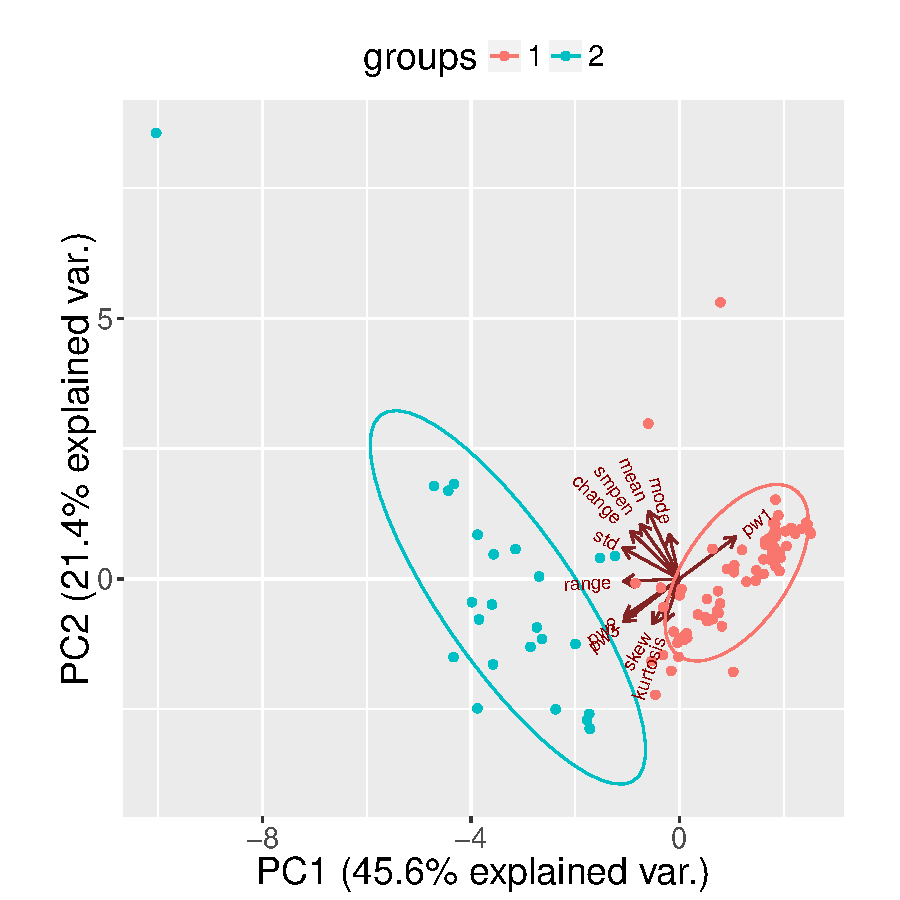
\includegraphics[width=.68\textwidth]{gfx/chap3/ping_pca_ping.pdf}
\caption{Projections of clusters on \ac{PCA} features, \texttt{PingData}.}
\label{fig:ping_pca}
\end{figure}

\marginpar{view from \ac{PCA} surface}
This ``guess'' can be straightforwardly observed from the projection of clusters on \acf{PCA} surface, shown in Fig.~\ref{fig:ping_pca}.
The contribution of each feature is as well indicated on the graph.
We notice that selected features point to different directions on the \ac{PCA} surface, suggesting that they contribute to a non-redundant description of the date set.
As a consequence, no single feature takes dominant position in forming the clusters.
Still, tendency is that cluster 2 includes data points with little  changes, small entropy and small standard deviation. 

\begin{figure}[!htb]
    \centering
    \begin{subfigure}[b]{\textwidth}
	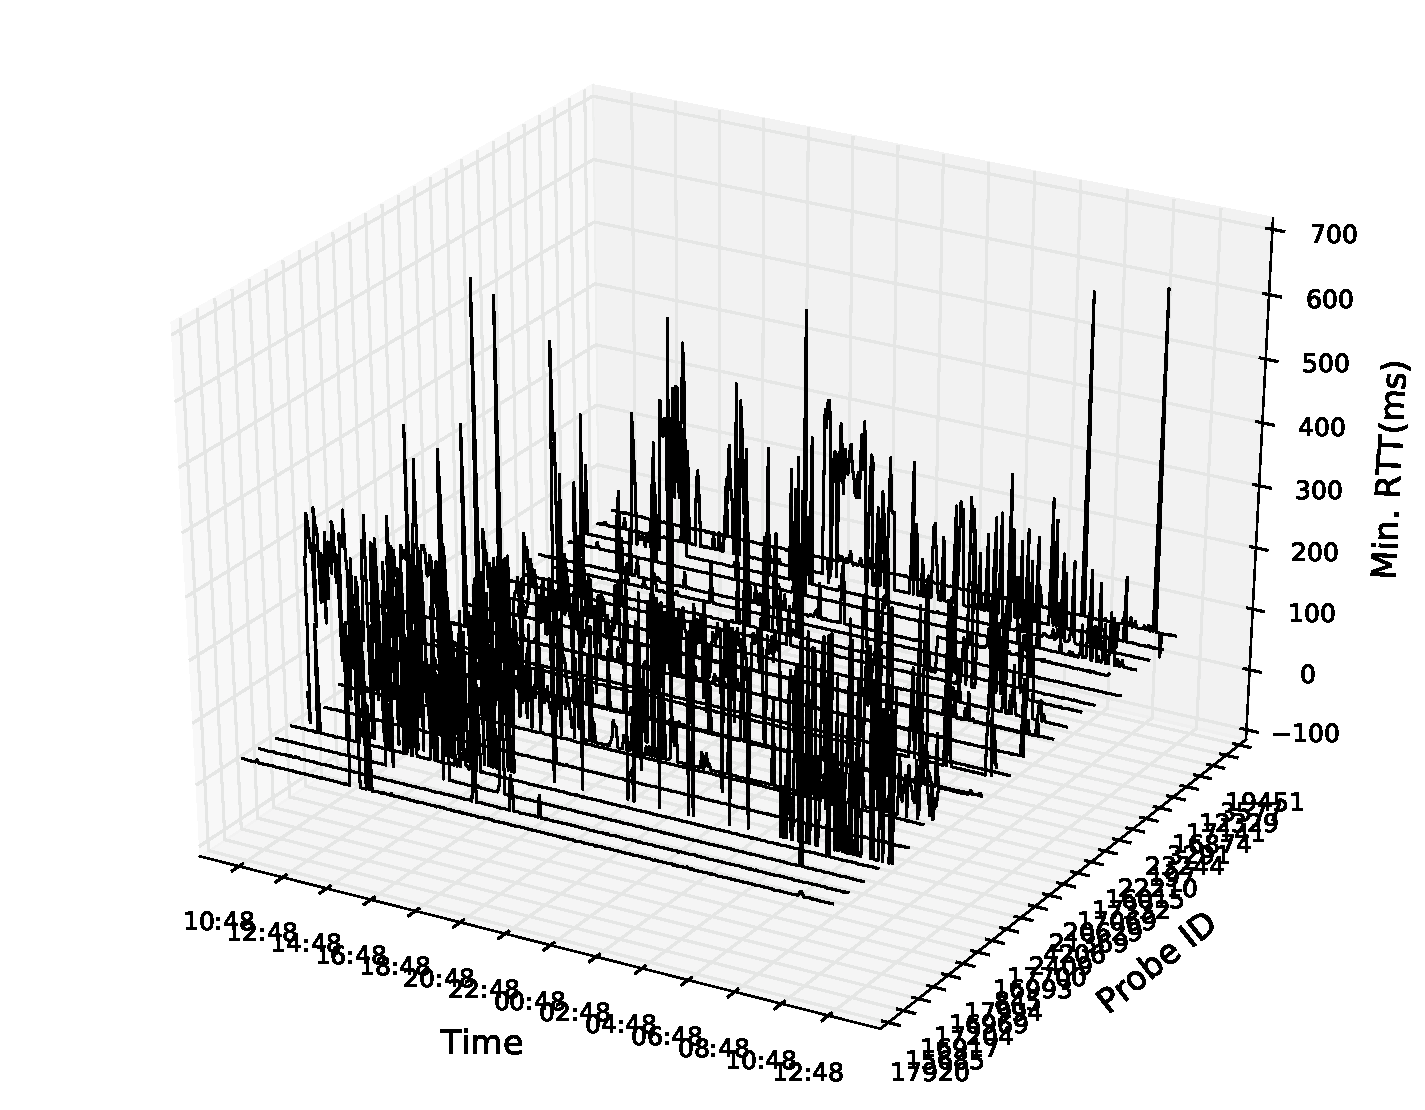
\includegraphics[width=\textwidth]{gfx/chap3/rtt3d_ping_cls1.pdf}
	\caption{cluster 1.}
	\label{fig:ping_cls1}
	\end{subfigure}
	\begin{subfigure}[b]{\textwidth}
	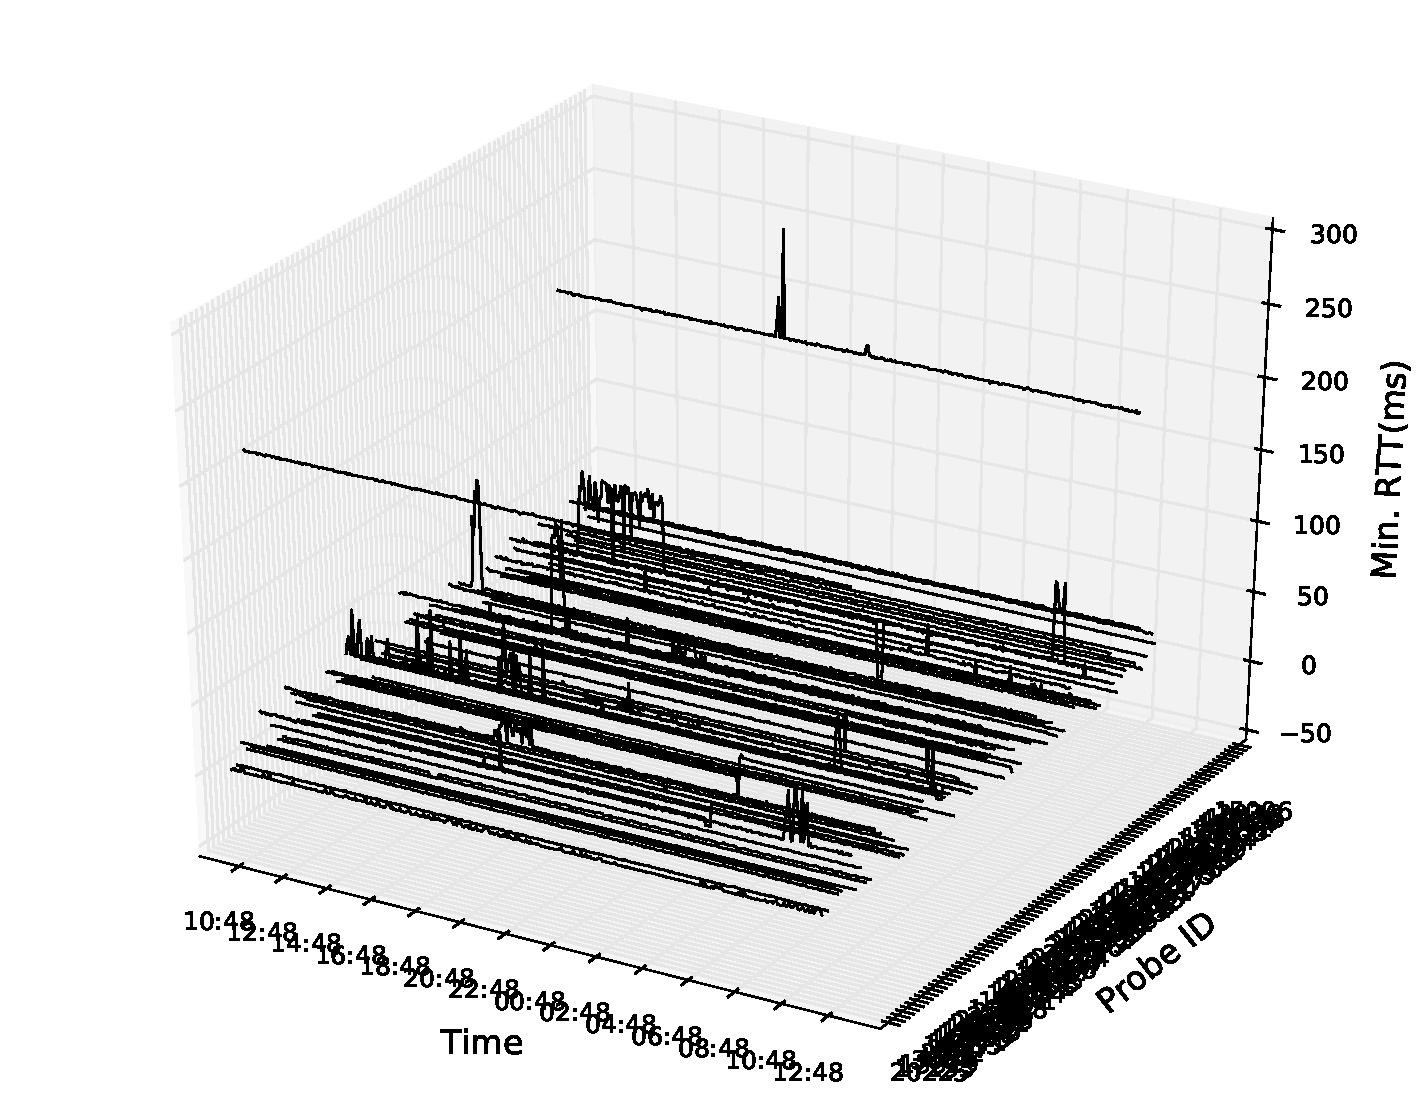
\includegraphics[width=\textwidth]{gfx/chap3/rtt3d_ping_cls2.pdf}
	\caption{cluster 2.}
	\label{fig:ping_cls2}
	\end{subfigure}
\caption{End-to-end RTT series of cluster members from \texttt{pingData} dataset.}
\label{fig:rtt_ping}
\end{figure}

\marginpar{view from RTT time series}
Fig.~\ref{fig:rtt_ping} plots the RTT time series of these two clusters. Cluster 2, as expected, contains mainly time series with only a few variations and spikes. 
On the other hand, cluster 1 is composed of traces with large variations.
This explains why the members of cluster 2 are more closely located to each other. 
It is because for a time-series to be smooth, there is only one form, while for it to be full of variations, there could be many possibilities.
%Let's also note that for smooth time-series (cluster 2), there is only one form, 
%while many different possible shapes can be observed in the other cluster.

\begin{figure}[!htb]
\centering
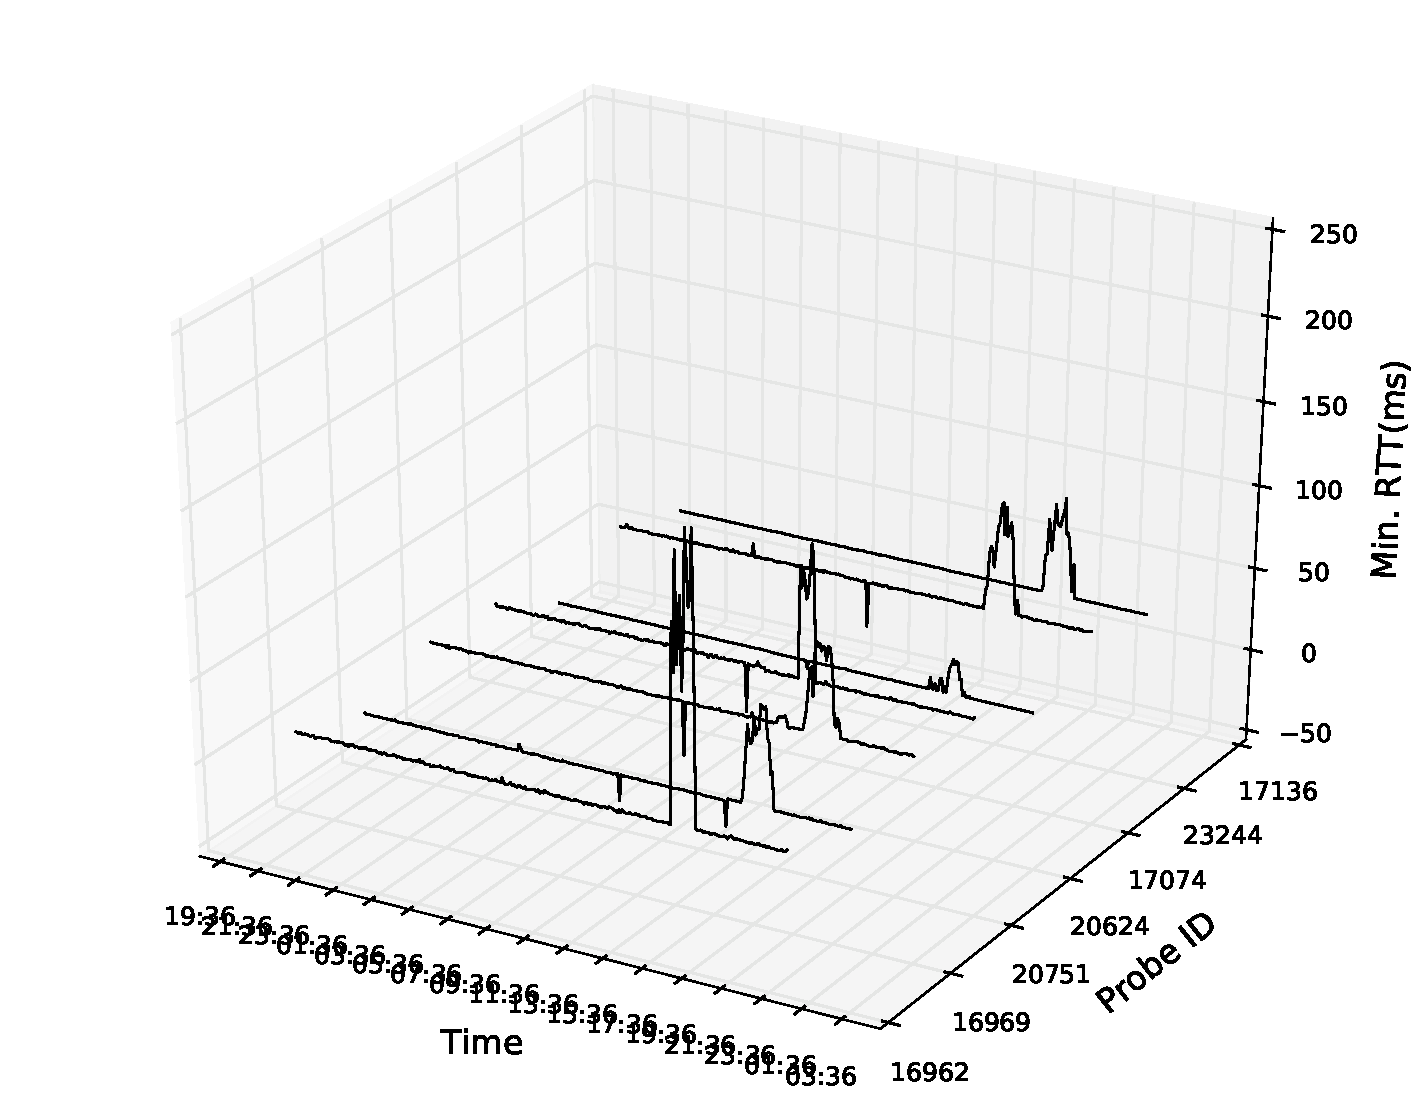
\includegraphics[width=\textwidth]{gfx/chap3/rtt3d_ft_pam_cls8.pdf}
\caption{One cluster achieved when $k=12$, \texttt{PingData}.}
\label{fig:cls8_k12}
\end{figure}

\subsubsection{Advantage of clustering}
What is also worthy of noticing is that cluster 2 actually tolerates traces with a few spikes and variation of small amplitude. 
This is due to the advantage of using clustering instead of ranking with one single feature, which would also be viable to filter out ``noisy'' traces. 
For instance, we could rank the RTT traces by their entropy and assume top x traces are ``noisy'' ones. 
The shorting-coming of such approach is two-fold.
First, single feature might ``wrongly'' rank certain RTT time series. 
For example, entropy~\cite{Molina-Pico2011} and power spectral density are very sensitive to spikes. 
In networking uses, we believe that one or a few spikes in an RTT measurement shall not deteriorate an entire measurement time series. 
Second, one has to define threshold values to deliberately separate data set into two or more parts. 
While with clustering, multiple features can be considered at same time. 
Plus, the most appropriate number of clusters changes automatically with the input and reveals the inherent structure of the data set. 
By setting a larger cluster number, one could achieve more fine-grained clustering results that convey subtler information. An example is given in Fig.~\ref{fig:cls8_k12}, where several traces of similar variation shape is grouped together.

\subsubsection{Implications for interdomain TE}
The two clusters achieved are as well of relevance in interdomain TE. 
It shows that when measuring an AS-level path by probing multiple hosts in the destination network, resulted RTT time series can take very different shapes. 
One possible explication is that the IP-level path toward certain hosts suffers from local problems.
If certain RTT variation is due to congestion on an inter-AS link, then it shall be shared by all the RTT time-series. If not shared, such RTT variation is probably related to local issues can not be avoided by changing an egress transit provider in sending out the traffic.
Therefore, when comparing multiple RTT time series between two ASes, the ones with fewer variations are supposed to be less impacted by these local conditions and give a more faithful view on the AS-level path performance.
One another advantage of using smoother RTT time series in choosing egress transit is that resulted routes are supposed to be more stable. as fewer variations should potentially trigger fewer route changes. 

\subsubsection*{Take-away}
To summarize, when clustering RTT time series in feature space, no specific assumption is imposed by the extracted features, yet we arrive at two clusters that tell noisy traces apart from smooth ones.
This reveals the inherent structure of the data set, that is for multiple RTT time series describing a common AS-level path, a majority of them resembles each other and demonstrates least variations possible, while a handful of ``outliers'' may exist that contain diverse additional variations. 
Considering the source of our data, our assumption is that some of the RIPE Atlas probes are continuously suffering from local system or access network conditions. 
%%%TODO: caption of table 1, feature space, explanation
%%% What is "feature space". not defined sorry. 

\subsection{Where do the RTT variations come from?}

\begin{table}[!htb]
\centering
\footnotesize
\setlength{\tabcolsep}{0.5em}
\begin{tabular}{l|cc|cc|cc}
\toprule
\multirow{2}{*}{\texttt{pingData}} & \multicolumn{2}{c|}{\texttt{traceData1}} & \multicolumn{2}{c|}{\texttt{traceData2}} & \multicolumn{2}{c}{\texttt{traceData3}}\\
 &  1 & 2 & 1 & 2 & 1 & 2\\
\midrule
1 & 25 & 0 & 8 & 17 & 20 & 5 \\
2 & 68 & 7 & 68 & 7 & 11 & 64 \\
\bottomrule
\end{tabular}
\caption{Comparing cluster members resulted from different datasets. The number in each cell represent the number of common members share by the two clusters.}
\label{tab:comp_cls}
\end{table}

In this part, we tried to find out the origin of these additional RTT variations in cluster 1 of \texttt{PingData}, and their practical meanings in networking.
To this end, we clustered the RTT time-series of the first 3 hops extracted from traceroute measurements, and compared the cluster members to the ones obtained from end-to-end ping measurements in Table~\ref{tab:comp_cls}.

We observed that for \texttt{traceData2} (hop 2) and \texttt{traceData3} (hop 3), not only the cluster sizes arrived are in accordance to those from \texttt{pingData}, but also a majority of cluster members overlaps. 
That is to say, using RTT series till the 2nd hop or the 3rd hop, we ended up with similar clustering results as with end-to-end RTT series. 
This observation is further confirmed by Table~\ref{tab:summary_cls}, which calculates some statistic measures on \texttt{pingData} feature space for clusters resulted from each dataset. 
Clusters from \texttt{traceData1} have the poorest overall \ac{ASW} indicating that its clusters are not a good fit for end-to-end RTT time series. 
However, clusters resulted from \texttt{traceData2} and \texttt{traceData3} seems to be quite OK on the feature space of \texttt{PingData}, as the overall \ac{ASW} is not far away from that achieved with \texttt{PingData} itself.
%Considering that clustering on the feature space can indeed group RTT time-series by their level of variance, shown in Fig.~\ref{fig:rtt_ping} and Fig.~\ref{fig:ping_pca},
As clustering results on end-to-end RTT and on RTT till the 
2nd and 3rd hop are highly similar, we are able to assume that most variations in the end-to-end RTT data set are expressed by the link between 1st and 2nd hop.

\begin{figure}[!htb]
\centering
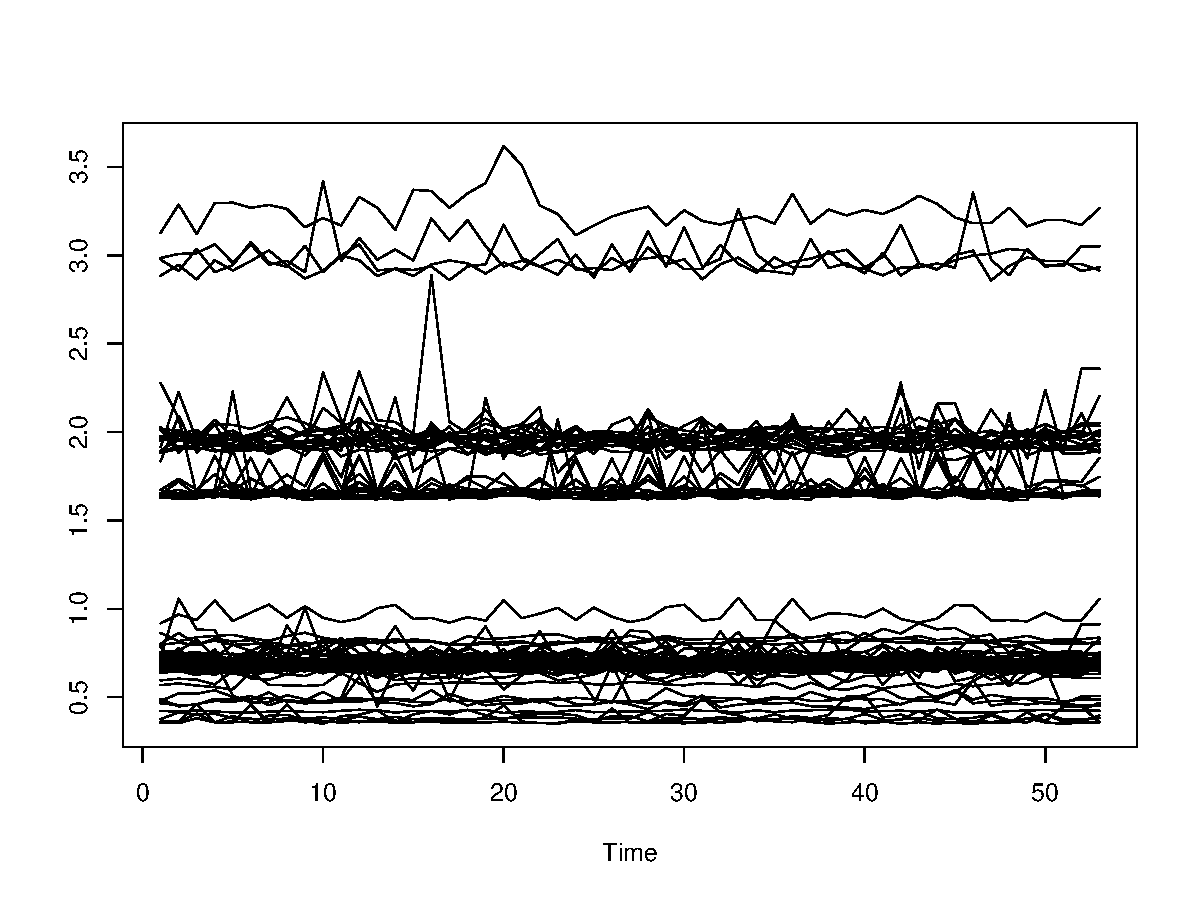
\includegraphics[width=\textwidth]{gfx/chap3/trace1_cls2_traceRTT.pdf}
\caption{RTT (in msec) till first hop. The first hop is assumed to be the hop till home router, yet three different baselines are observed. This might due to differences in connection methods, hardware and firmware versions of Atlas probe and ISP home router.}
\label{fig:trace1_traceRTT}
\end{figure}

In this specific case, where the probes involved are within the residential network of an ISP AS3215, the first hop probably arrives at the home router. This guess is indirectly confirmed by the observation that most traceroute records has \texttt{192.168.1.1} as the first hop address. As expected, RTT traces till the first hop are all generally pretty smooth according to Fig.~\ref{fig:trace1_traceRTT}. We manually searched second hop addresses, e.g. \texttt{80.10.127.143} in \url{https://db-ip.com/80.10.127.143}. Results returned show that they are all access equipment of the ISP.
It is thus logical to find most variation between the 1st hop (home router) and the 2nd hop (ISP access equipment), as it corresponds to the ISP access network.  

Such finding is of course not a huge surprise.% but rather a common sense among network engineers. 
However, it suggests that with our clustering method, we are able to get rid of RTT measures that undergo severe access network problems. 

\subsection*{Wrap-up}
In this study, we date-mined RTT time series between two ASes. 
We found out that RTT time series collected in this study demonstrate diverse variation shapes though one common AS path is measured.
It confirmed that RTT measurements need to be ``cleaned''.
We clustered these RTT time series by extracting %a couple of 
several features as their data representation. 
Resulted clusters successfully separate noisy traces from smooth ones according to human intuition and expertise.
Furthermore, we located the occurring location of most variations in end-to-end RTT measurements by applying the presented clustering methods to the first hops of traceroute measurements.
Our results confirmed the common sense that most variations come from the access network.

\section{Multiple RTT time series with synchronized changes}
\label{sec:ripe_case_study}

A case, illustrated in Fig.~\ref{fig:cls8_k12}, where multiple RTT measurements undergoing at the same time a similar shape RTT variation, intrigues us a lot. This RTT change is not observed on other RTT measurements, which indicates that a common part exclusive to these RTT measurements in Fig.~\ref{fig:cls8_k12} could have caused this change.
Capable of inferring the location where RTT changes in the Internet happen from readily available delay and path measurements on the client TE platform offers precious visibility that might contribute to better route selection logic.

Clustering in feature space (Section~\ref{sec:cls_ft}) is however not an appropriate approach for the identification of RTT time series with similar shapes, because the features extracted, summarizing the entire time series, do not have the capability conveying information concerning temporal structure.
Therefore, we study the clustering approaches where the data representation of RTT time series remain time series.

\subsection{Data collection}
\marginpar{collection}
In order to increase the chance of identifying RTT time series with shared change or shape, We collected ping and traceroute measurements from 170 RIPE Atlas probes hosted in European datacenters to DNS b-root from Jan.\ 18 to Jan.\ 24, 2016\footnote{DNS b-root had single single instance at that moment.}\footnote{IDs of these probes can be found at \url{https://www.dropbox.com/s/6ai0aooxnubufma/pbid.txt?dl=0}.}.
We cleaned the dataset by removing measurements with plenty of missing segments and timeout measurements.
128 probes remained. They are from 17 countries, 117 ASes and 120 prefixes. All these probes are equipped with the lasted v3 hardware.

\marginpar{pre-processing}
The measurements from different Atlas probes are not strictly aligned.
This brings inconvenience in analysis that compare RTT changes across probes. 
We therefore found a set of new timestamps for ping measurements that minimizes the average distance from initial measurement timestamps to it.
The resulted average time distortion from the new timestamps to initial ones is $55.01 sec$, being much smaller than the measurement interval, i.e.\ $240s ec$.
We henceforth aligned the initial RTT measurement measurements to the closest new timestamp.
For several rare moments when no measurement data was available, we padded them with closest RTT measurements.
Hence, we achieved a dataset with aligned timestamps and equal length.

\subsection{Data representation}
In order to capture the temporal structure of time series, we tired following data transformations that result still in time series.

\paragraph*{Raw RTT}  The aligned and padded raw RTT measurements are used as them are for the sake of comparison. This representation is denoted as \textbf{RTT} later on.

\paragraph*{Segments by changepoint detection} In the purpose of filtering unnecessary variations in the raw RTT measurements, we applied changepoint detection to them. The operation cuts each RTT time series into segments of different characteristics. We then simplify each RTT time series with the mean value of each segment without changing its total length. So achieved time series are denoted as \textbf{Seg}. The changepoint detection is performed with R package \textit{changepoint}, version 2.2.1~\cite{Killick2013a}. The min RTT is first subtracted from each RTT time series. Then we assume Poisson distribution during the change detection. We later on dedicate  Chapter~\ref{sec:cpt_rtt} to the change detection for RTT measurements, where more technical details can be found.

\paragraph*{Z-normalized time series} This process produces zero mean unite variance time series. It is a very common data pre-processing in time series clustering~\cite{Ulanova2015,Ratanamahatana2004}. It helps remove the difference among RTT measurements caused by level difference that is less relevant to shape. However, it as well cause RTT time series with large change amplitudes to resemble a lot those with small variations, and make them indistinguishable. Due to this undesired feature, the actual clustering result with z-normalized time series is relatively meaningless. Therefore, we no longer discuss this data representation.

\paragraph*{Mode-centered and piece-wise scaled time series}  In this transformation, we first center each RTT series around its mode by:
\begin{align*}
x_m = x-\tilde x,
\end{align*}
where $\tilde x$ is the mode of time series $x$. Then we scale the $x_m$ time series by the following piece-wise function:
\begin{align*}
F_s(x) =
\begin{cases} 
       0    \hfill & \text{$0 \geq |x| < 10$}, \\
       x-10 \hfill & \text{$10 \geq |x| < 60$ }, \\
       10 \times \log_2 (|x_i|) - \beta \hfill & \text{$|x|\geq 60$},\\
  \end{cases}
\end{align*}
where $\beta = 10 \times \log_2 60 - 50$, being simply a term to make the $F_s(x)$ continuous in value. 
The intuition behind these operations are 1) since networks tend to have a dominant configuration and are most of the time free of congestion, it is variation around the most popular value that defines the shape of the RTT time series; 2) for little variations less than 10 msec, we would like to consider them as insignificant noises and filter them; for moderate deviations, say in the range of $[10 msec, 60 msec)$, are changes that we would like to take into account during clustering thus conserved linearly; while for super large changes, sometimes outlier values, greater than 60 msec, we would like to suppress their impact on clustering results. We refer to resulted time series as \textbf{MP}.

\subsection{Distance measure}
Wang et al.\ \cite{Wang2013} performed a comprehensive study on distance measures for time series data. They showed no distance measure is significantly better (in terms of the accuracy finding 1 closest neighbour) than \acf{DTW} on a majority of data studied \cite{UCRArchive}, while \ac{ED} is of similar performance as \acf{DTW} when training sample are big enough. Therefore, we consider these two well studied distance measures.

\paragraph*{Euclidean Distance} is a non-elastic distance measure, which can only be applied to two time series of same length. For $x$ and $y$ of length $N$, ED is defined as:
\begin{align}
ED(x,y) = \sqrt{(x_1 - y_1)^2 + (x_2 - y_2)^2 + \dots + (x_N - y_N)^2}.
\end{align}
All the above presented data representation contain time series of same length, thus applicable.

\paragraph*{Dynamic Time Wrapping} is an elastic distance measure, which allows it to handle time series of different length. Yet, \cite{Ratanamahatana2005} showed that there is no significant difference in terms of classification accuracy for \ac{DTW} in handling time series of different length and re-interpolated series of same length. 
Therefore, padding shall bring few impact when employing \ac{DTW}.
Different from ED, \ac{DTW} stretches or compress the two time series so that one resembles the other as much as possible. That is, one value in a time series can be aligned/matched to one or multiple values of arbitrary positions in the other time series, so that the accumulated distance between all aligned/matched points are the smallest. Constraints exist in finding such alignment, or in other words wrapping path, the details of which can be found in \cite{Sakoe1978, Keogh2005, Giorgino2009}.

\begin{figure}[!htb]
\centering
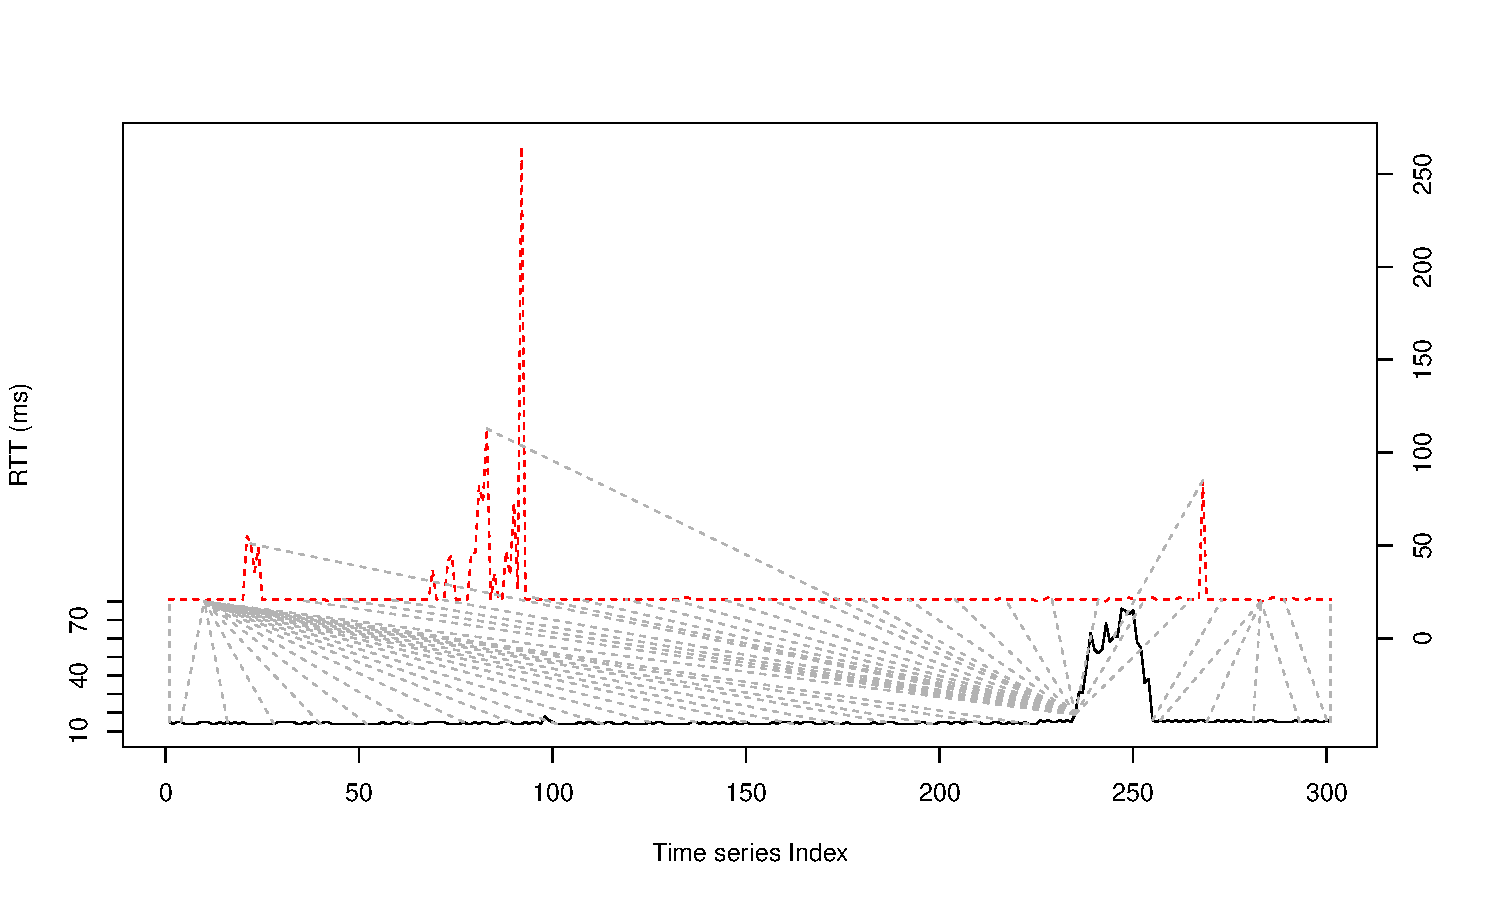
\includegraphics[width=.8\textwidth]{gfx/chap3/dtw_ex.pdf}
\caption{Matching/aligning of two RTT series. The black line is the query series, probe id 16969; the red dashed line is the reference series, probe id 16987. Dashed lines between these two series illustrates how values in query is matched to ones in the reference. The distance resulted is 3457.}
\label{fig:dtw_ex}
\end{figure}

Fig.~\ref{fig:dtw_ex} gives an example of how \ac{DTW} aligns a query RTT series to a reference series. We can see that the RTT variation of the traces happen in times far apart from each other. However, with \ac{DTW}, these variations are sort of aligned. The advantage of this feature is that \ac{DTW} can identify shape similarities that are not aligned in time.

\begin{figure}[!htb]
\centering
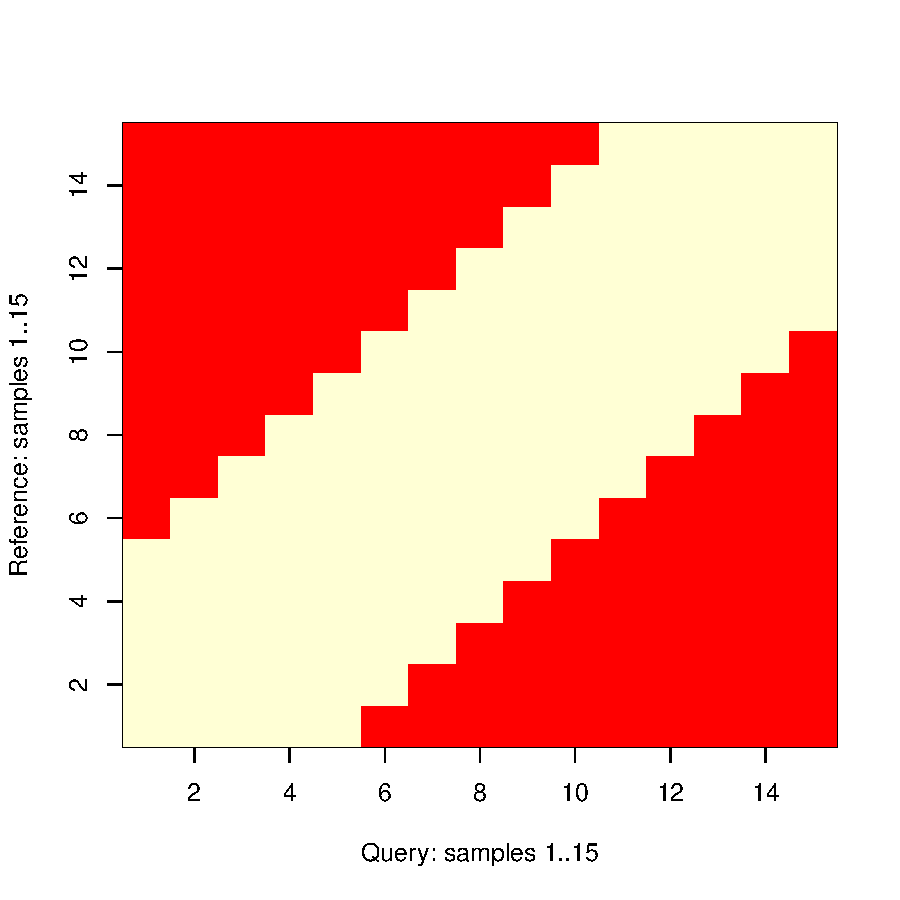
\includegraphics[width=.5\textwidth]{gfx/chap3/win.pdf}
\caption{A Sakoechiba  window \cite{Sakoe1978} of 4 in size. Yellow part is the allowed alignment/matching area.}
\label{fig:win}
\end{figure}

\begin{figure}[!htb]
\centering
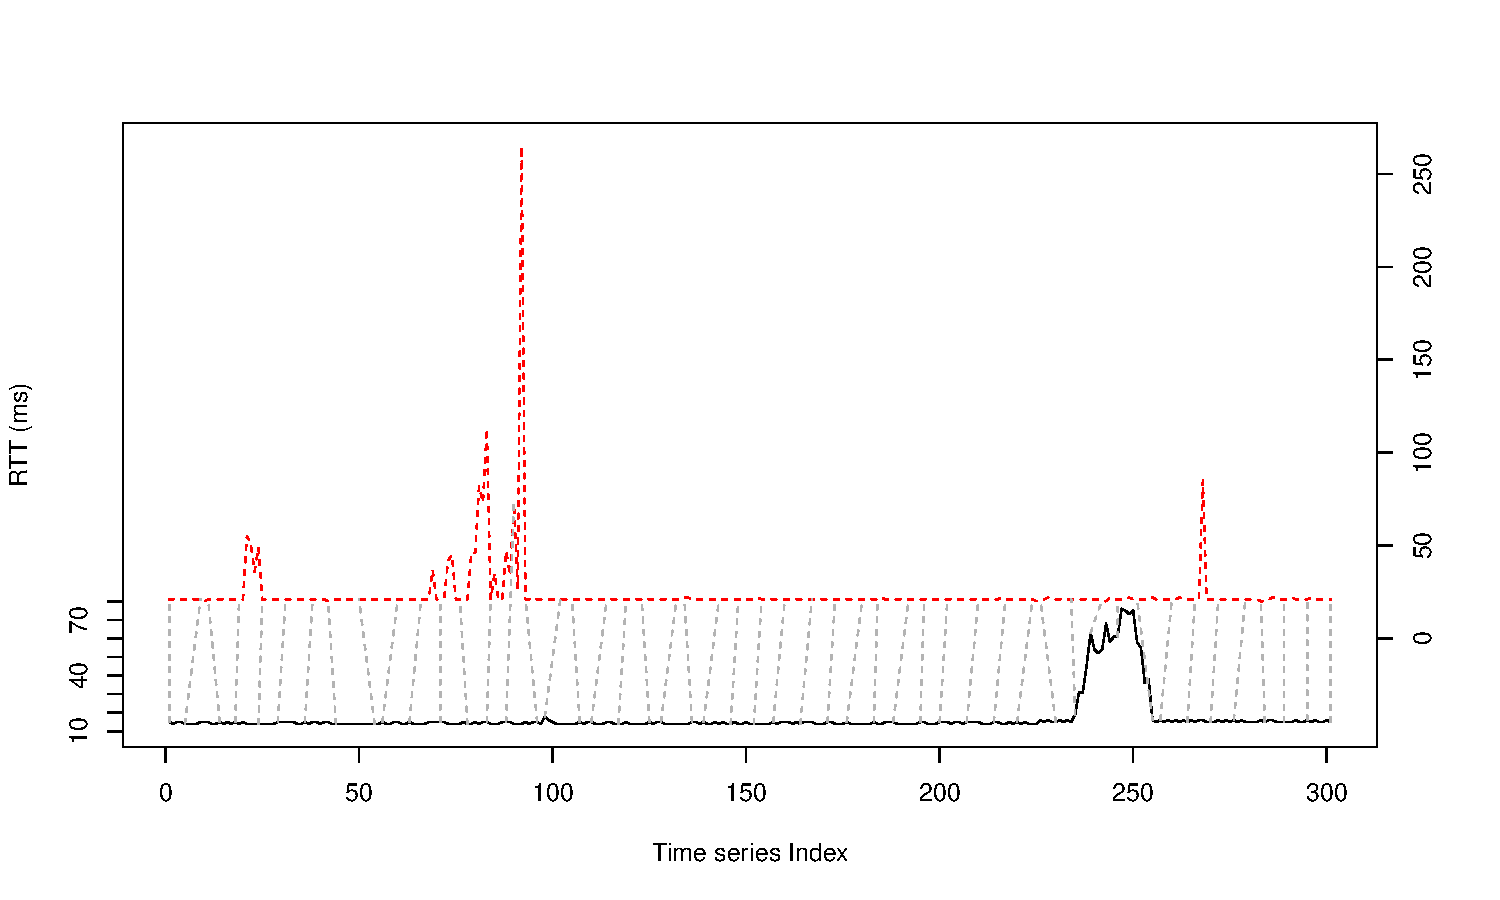
\includegraphics[width=.8\textwidth]{gfx/chap3/dtw_ex_win.pdf}
\caption{Matching/aligning of two RTT series with window. The black line is the query series, probe id 16969; the red dashed line is the reference series, probe id 16987. Dashed lines between these two series illustrates how values in query is matched to ones in reference. The distance resulted is 5181.}
\label{fig:dtw_ex_win}
\end{figure}

However, matching variations far away in time as is the case in Fig.~\ref{fig:dtw_ex} dosen't really help in finding synchronized changes, which is of interest to us. Therefore we apply a window restricting the range of alignment/matching between two RTT time series. The window used is visualized in Fig.~\ref{fig:win}. With window size equaling 4, a data point in one time series can no longer be match to a point 5 index further in the other series. 5 index in our RTT measurements, means 20 min, which is already a large range. With the window, the new alignment is shown in Fig~\ref{fig:dtw_ex_win}.

\subsection{Clustering results}

\marginpar{justify the use of \ac{PAM} as clustering algorithm}
We used \ac{PAM} instead of k-means because 1) \ac{PAM} is more robust than k-means, for its clustering result is less impacted by outlier observations~\footnote{The only difference between \ac{PAM} abd k-means lies in that k-means uses the mean value of cluster members as the prototype of that cluster, around which the cluster member are iteratively adjusted, while \ac{PAM}, a.k.a. k-medoids uses the cluster member that minimizes the total distance between itself and all other cluster members as the cluster prototype.}.
2) the mean 'value' of a set of time series does not have any practical meaning, while the medoid is a common choice~\cite{Aghabozorgi2015}. 

The clustering result with \ac{ED} is relatively not meaningful, and will not be discussed later on. It forms one cluster containing a majority of RTT time series without observably similarity among them, and several small clusters having strictly matched RTT spikes. We believe it is because the distance definition is too stiff .

\begin{figure}[!htb]
\centering
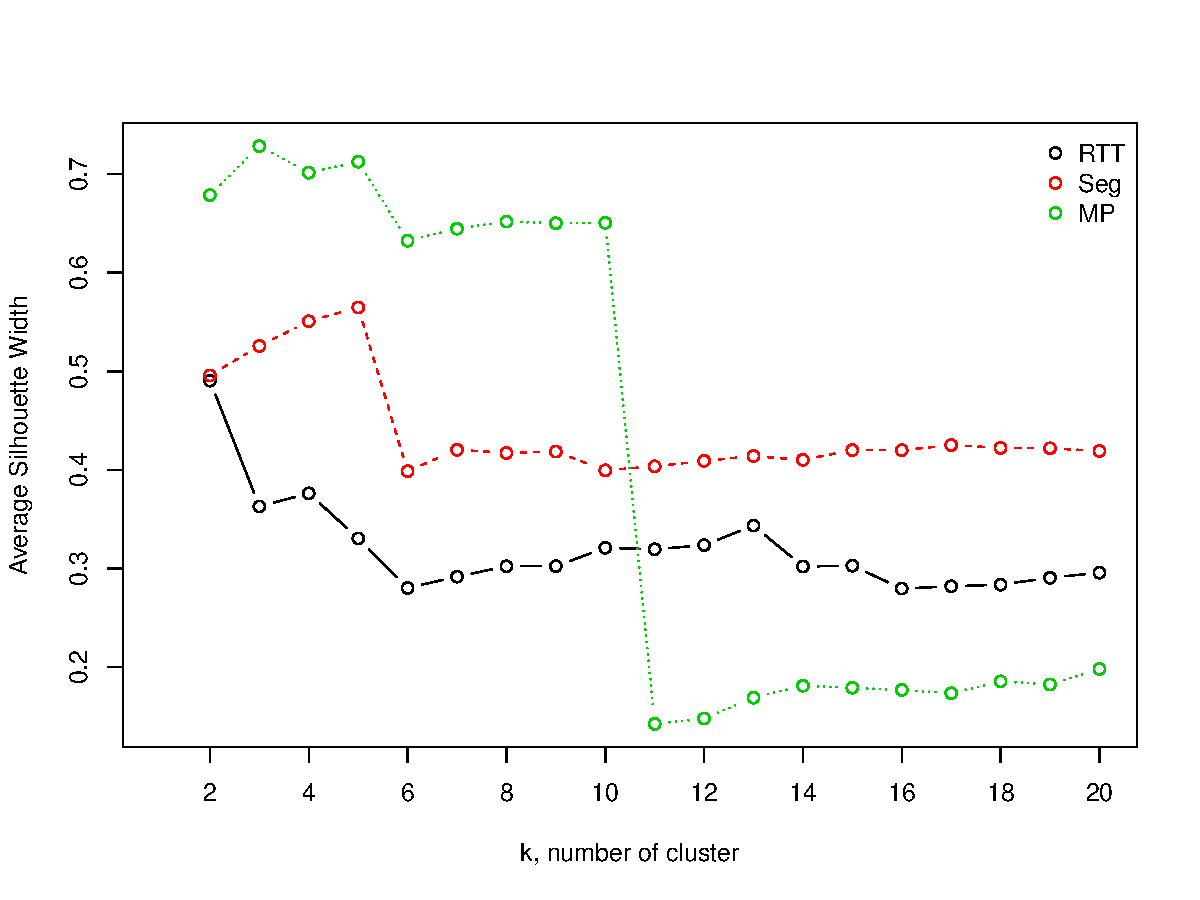
\includegraphics[width=.8\textwidth]{gfx/chap3/sil_comp.pdf}
\caption{\ac{ASW} over the entire data set with varying k.}
\label{fig:sil_comp}
\end{figure}
We thus mainly compare the clustering results using \ac{DTW} and \ac{PAM} over the three data representations: \textbf{RTT}, \textbf{Seg} and \textbf{MP}. The \ac{ASW} with varying cluster number k is given in Fig.~\ref{fig:sil_comp}. The curve for \textbf{MP} demonstrates a very typical step-wise shape, evidence of strong cluster structure when $k \leq 10$. Among the three representations, the clustering algorithm is most confident of the clusters identified for \textbf{MP}.

\begin{figure}[!htb]
\centering
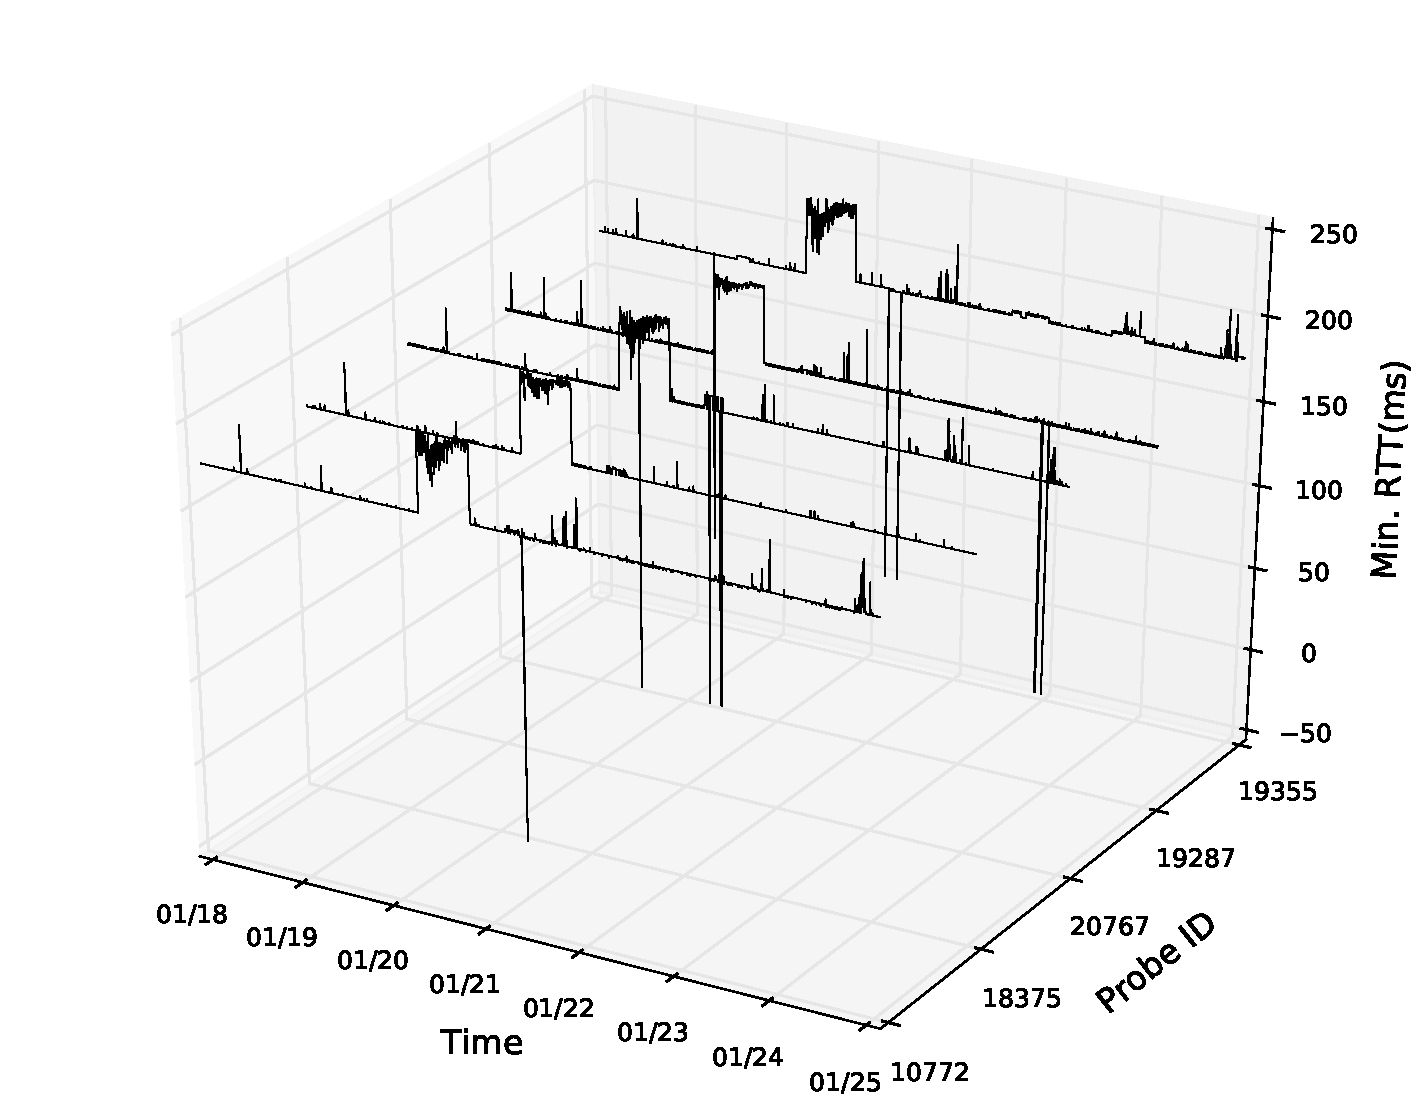
\includegraphics[width=.9\textwidth]{gfx/chap3/rtt3d_mp_cls2.pdf}
\caption{A common cluster in \textbf{MP} and \textbf{Seg} when $k=5$.}
\label{fig:rtt3d_mp_cls2}
\end{figure}

Investigating RTT time series of resulted clusters, we found that RTT time series in \textbf{RTT} are essentially grouped by their RTT level, indicating the meaning value of raw RTT time series dominates the distance calculation. \textbf{MP} and \textbf{Seg} contain pretty similar clusters when the \ac{ASW} is relatively high for both data representation at $k=5$. One cluster containing exactly the same member RTT time series under both representations is shown in Fig.~\ref{fig:rtt3d_mp_cls2}. With both representation methods, a almost 0.8 \ac{ASW} is achieved for this cluster, meaning that the clustering algorithm is extremely certain about this result. Other clusters of \textbf{MP} and \textbf{Seg} are as well of relevance, indicating they are very effective ways of extracting temporal structures in time series.

\subsection{Network implications of shared RTT variation}

The 5 RTT time series in Fig.~\ref{fig:rtt3d_mp_cls2} experienced a big RTT increase of at least $40msec$ for nearly a day on Jan. 20th, 2016.

\marginpar{What happened?}
\paragraph*{Common AS hop} The only intermediate AS shared by all the 5 probes is AS6939.
Meanwhile, other 94 probes in our dataset that pass through AS6939 didn't experience this RTT change.
3 of the 5 probes pass through IXP AS8674, right before entering AS6939.
The other 2 have unannounced IP addresses interconnecting AS6939.

\paragraph*{Routing changes} No AS path change is witnessed during this period.
However, there are IP level path changes within AS6939 happened at the same moment as the shared RTT changes~\footnote{We are capable of distinguishing real IP path changes and those due to \ac{LB}, more technical details in Section~\ref{sec:cpt_rtt}.}.
RTT till the hop entering AS6939 experienced the most significant increase when inspecting the traceroute measurements.

\paragraph*{Possible scenario} Our guess was that IXP AS8674 changed the next-hop in reaching AS6939 out of some reason and the impacted traffic fell on a congested inter-AS link.
The \acf{NOC} team of AS8674 kindly replied to our query and told us that they did ``not see any special disturbance''. 
Another possibility is that due to \acf{NDA}, they were not allowed to reveal any information to non-member entities.
In both cases, it turned out to be very difficult to identify which part of the Internet causes the shared change, using merely end-to-end measurements.
Yet, capable of clustering in first place RTT time series with similar shapes does help narrow down the scope of possible causes.

\subsection{Limitations of time series clustering}

Time series clustering with \textbf{MP}/\textbf{Seg} and \ac{PAM} offered very interesting results and helped us chasing down a specific case of RTT change shared by multiple RTT time series.
However, it is still not ideal in the context of measurement-based TE for following reasons.

First, it won't scale. In order to obtain a distance matrix among $n$ time series, $O(n^2)$ distance calculation is needed. The computation cost for clustering could thus be prohibitively high when there are thousands of RTT time series, one for each destination prefix. 

Second, the interpretation of clustering results remain ad hoc, and thus hard to be automatized. \ac{ASW} of each cluster can serve as an indicator of cluster quality/relevance. Yet, what level of \ac{ASW} should be considered significant enough is hard to justify. In previous analyses, we always resorted to raw RTT time series to judge if the clusters are indeed meaningful or not, before carrying out more specific analysis. On top of that, the clustering results do not state when RTT changes shared by the cluster members actually happen, preventing as well systematic investigation of relating network events at these moments to infer the causes of the RTT changes.

Third, it is hard to transform clustering into an online process. Along the time, different parts of the Internet might cause RTT changes, impacting different sets of RTT measurements, hence different clusters over time. This requires the clustering methods to update the resulted clusters as new measurements flow in. This is not what clustering methods studied in this chapter are capable of.

To address the above issues, we found simplifying RTT time series via changepoint detection promising. It first outputs the moments when each RTT time series experiences significant changes. Based on this change-or-not binary status, we can then easily form groups of time series sharing the same change. With evolving groups, we can track the causes for different RTT changes over time in the Internet.
We develop this idea in Chapter~\ref{sec:cpt_rtt} and ~\ref{sec:infer}.
